\section*{\centerline{ВВЕДЕНИЕ}}
\addcontentsline{toc}{section}{ВВЕДЕНИЕ}
Быстрое развитие промышленной автоматизации обусловило развитие методов и средств сбора данных и управления, начиная с всевозможных датчиков и заканчивая SCADA-системами. С развитием SCADA-систем возникла необходимость учёта и контроля многих узлов системы, не привязанных к измерительному оборудованию. Для обхода данного препятствия были задействованы беспроводные технологии: Wi-Fi, RFID, датчики определения местоположения объекта. В работе рассматривается внутренняя структура и алгоритм работы устройства определения расстояния между объектами методом \textit{Time of Flight}.

Радиолокация --- область науки и техники, объединяющая методы и средства локации (обнаружения и измерения координат) и определения свойств различных объектов с помощью радиоволн~\cite{wiki:radiolocation}.

Радиолокация позволяет использовать радиоволны для автоматизации различных целей и задач, в том числе --- автоматизации производств, АСУТП-систем и SCADA. Например, используя специальные <<радиометки>>, закрепляемые на движущихся объектах, можно отслеживать пути перемещения различного технологического оборудования, заготовок на складах и даже передвижение персонала.

В то время, как GPS, ГЛОНАСС и подобные системы позволяют отслеживать перемещение объекта на открытой местности, они не позволяют отслеживать его внутри помещений. Всвязи с этим, в современных условиях промышленной автоматизации стоит задача создания систем отслеживания местоположения всех критических объектов внутри цехов.

Простейшая задача радиолокации сводится к вычислению расстояний между тремя точками, а затем вычислению местоположения специализированными алгоритмами (например, методом триангуляции). Дипломная работа сфокусирована на определении расстояния между двумя точками методом \textit{Time of Flight}, а также расчётё погрешностей и задержек, возникающих во время измерения, и, как следствие, разрешающей возможности конечного устройства в зависимости от выбранного оборудования.

% Постановка задач исследования.
% Описание объекта автоматизации.
% Цели.
% Обзор существующих аналогов.
% Обзор литературы по теме.

\section{РАДИОДАТЧИКИ В ДИСПЕТЧЕРСКИХ СИСТЕМАХ}
В контексте автоматизации определение местоположения объекта обеспечивает более гибкое управление технологическим процессом (например, в составе SCADA-систем).

Существуют следующие применения радиометок:

\begin{itemize}
    \item отслеживание объектов на складах: пометив каждый объект <<радиометкой>>, организация получает возможность быстрого нахождения нужного предмета, экономно сокращая время и ресурсы машин; становится реальной возможность быстрого подсчёта продукции на складах без необходимости хранения данных в сложных базах данных;
    \item отслеживание движения механизмов и объектов на конвейерах: благодаря данной возможности, можно строить модели передвижения и работы всей текущей системы в целом, улучшать производительность и экономичность данной системы;
    \item отслеживание движения рабочего персонала (управление предприятием): позволяет исключить простой рабочего времени и с точностью определить график времени рабочего.
\end{itemize}

В целом, радиометки улучшают качество и безопасность автоматической системы управления.

В зависимости от конкретных целей использования радиометок, задача обеспечения необходимой точности будет различаться. Например, для определения текущего местоположения накопителя или грузовика во дворе, будет достаточной точность в пределах 2-3 метров. Однако, для определения точной ячейки на складе хранения валов диаметром 30 см, нужна будет сантиметровая точность. Вместе с точностью растут и требования к конечному устройсту, такие как \textbf{частота работы}. Помимо высокой частоты, устройство должно использовать свободный частотный диапазон: например, 433 МГц или 2.4 ГГц (Wi-Fi).

С развитием промышленной автоматизации, крупные компании заметили преимущества SCADA-систем и стали использовать их для сбора, анализа и отображения информации с датчиков, а также корректирования дальнейшего управления на основе этой информации. Используя <<радиометки>>, система может корректировать регулирование на основе пространственного положения объекта, что увеличивает гибкость и надёжность системы.

Архитектура применения радиометок в SCADA-системе представлена на рисунке~\ref{fig:scada}.

\begin{figure}[ht]
    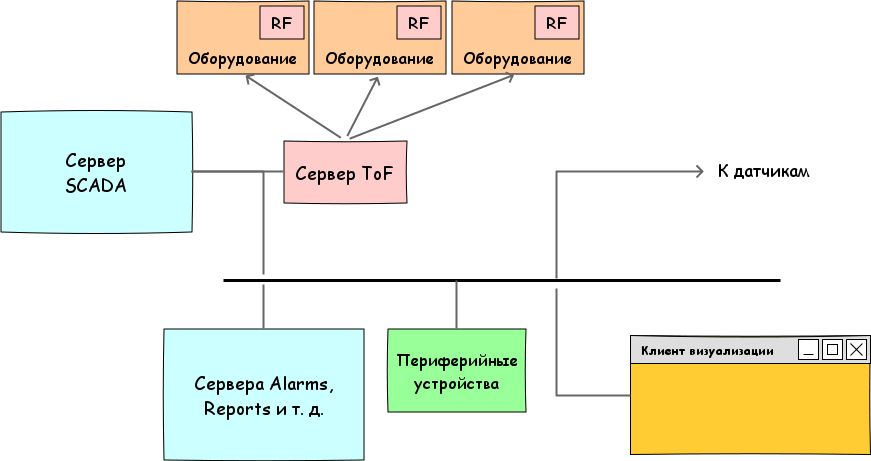
\includegraphics[width=1\linewidth]{Figures/scada.png}
    \caption{Применение радиометок в SCADA-системе}
    \label{fig:scada}
\end{figure}

Здесь RF - радиометка, отвечающая на полученное сообщение заданным сигналом (по запросу опрос-сервера).


    \subsection{Обзор существующих методов локализации}
    Есть несколько способов определения местоположения объекта:

\begin{itemize}
    \item ультразвуковые (sonic) устройства: просты в исполнении, однако на практике требуют прямой видимости между измерителем и объектом, что сокращает область применения;
    \item радиочастотные, методом определения уровня сигнала: не требуют больших ресурсов, однако точность такого измерения невелика: такой метод (RSSI) интерферирует с другими радиосигналами и ослабляется, отражаясь от препятствий;
    \item радиочастотные, прямой связью (метод \textit{Time of Flight}) между устройствами: измеряя время пролёта электромагнитной волны от передатчика к приёмнику и обратно, можно получить относительно точное измерение в рамках рабочей частоты устройства.
\end{itemize}

\subsubsection{Индикация уровня принимаемого сигнала}

Ультразвуковые и другие решения в большинстве случаев не подходят ввиду сложности помещений, цехов, складов. Наиболее простым способом измерения расстояния является метод \textit{Received Strength Signal Indication (RSSI)}. Любой беспроводной канал по стандарту IEEE 802.15.4 имеет протокольную функцию оценки качества связи (Link Quality Indicator), действие которой сводится к определению мощности принятого сигнала. Результат этого измерения можно вывести, откалибровать по известному расстоянию и оценить дальность до источника. Измерение расстояния производится следующим образом. Приемник с логарифмической амплитудной характеристикой принимает сигналы, по которым встроенный индикатор RSSI формирует 8-разрядный код RSSIVAL. Этот код получается в результате усреднения по восьми периодам (128 мкс) принятого сигнала и снабжается битом состояния, указывающим, когда RSSIVAL является валидным (т. е. приёмник имел возможность принять по крайней мере восемь периодов). Мощность принятого сигнала Р (дБм) вычисляется по формуле~\eqref{eq:rssi}:

\begin{equation}
    \label{eq:rssi}
    P = RSSI_{VAL} + RSSI_{OFFSET},
\end{equation}

где $RSSI_{OFFSET}$ — эмпирически подбираемая постоянная (порядка -45 дБм).

В идеальных условиях мощность обратно пропорциональна квадрату расстояния, логарифм мощности пропорционален расстоянию с некоторым коэффициентом, который устанавливается также эмпирически. Данный подход реализован в микроконтроллерах ZigBee фирмы TI серии CC2431.

Однако этому методу присущ ряд существенных ограничений, поскольку уровень сигнала является весьма изменчивым параметром из-за влияния следующих факторов:

\begin{itemize}
    \item быстрые и медленные замирания сигналов на трассе из-за изменения условий распространения радиоволн;
    \item многолучевое распространение вследствие отражений от различных металлических предметов;
    \item разброс выходной мощности передатчиков и чувствительности приёмников;
    \item влияние ориентации антенн из-за неравномерности диаграммы направленности.
\end{itemize}

Из-за воздействия указанных факторов реальная зависимость мощности от расстояния оказывается нелинейной и непостоянной во времени, вследствие чего точность измерений быстро падает с ростом расстояния. 

\subsubsection{Time of Flight}

Другой подход основан на измерении времени прохождения (пролета) сигнала (Time of Flight). Роутер посылает запрос на другой узел, получает ответный сигнал и определяет время его задержки. Полная задержка складывается из аппаратных задержек при обработке принятого и формировании ответного сигналов и времени распространения между узлами. Поскольку технические задержки известны с хорошей точностью, то их можно вычесть из полного значения, и оставшаяся величина будет характеризовать время пролета сигнала туда и обратно. Умножив половину времени задержки на скорость света, получим расстояние между узлами сети. В этом методе обеспечивается линейная связь между расстоянием и измеряемой величиной, и абсолютная точность измерения не зависит от расстояния. Для повышения точности используют многократные повторения процедуры измерения. Реально этот метод эффективен в полном диапазоне дальности работы сети (обычно сотни метров).

При качественной реализации, метод Time of Flight выигрывает у своих соперников почти по всем параметрам. Радиометки достаточно невелики и могут размещаться на объектах не занимая большого объема в отличие от ультразвуковых систем, которые занимают определённое место своим оборудованием.
 

    \subsection{Постановка задачи}
    Метод \textit{Time of Flight} заключается в измерении времени полёта электромагнитной волны от источника к приёмнику и обратно. На основе этого осуществляется расчёт расстояния между двумя точками. \textit{Time of Flight} применяется внутри помещений с большим количеством <<радиометок>>, где необходима большая точность. Однако, с точностью растут и необходимые требования к конечному устройству.

Всвязи с этим, ставятся следующие задачи:

\begin{itemize}
    \item устройство должно работать на относительно высокой стабильной частоте: для точности измерения в 1 метр частота работы должна быть 300 МГц;
    \item необходима точная синхронизация времени: расхождение начального отсчёта времени источника и приёмника значительно скажется на результате измерения;
    \item мельчайшие шумы будут сказываться на результате, уменьшая точность измерения;
    \item необходимо учитывать всевозможные задержки оборудования, а также возможные отклонения генераторов тактовой частоты друг от друга, т. к. \textit{Time of Flight} очень чувствителен к погрешностям: маленькие отклонения времени дают большие отклонения расстояния;
    \item необходимо разработать быстрый и стабильный протокол общения передатчика и приёмника друг с другом.
\end{itemize}

В конечном итоге, необходимо выбрать оборудование с минимальными задержками, вычислить постоянную аппаратную задержку и описать программную модель измерения расстояния методом \textit{Time of Flight}.

Для устранение ошибки рассинхронизации <<часов>> приёмника и источника применяют метод \textit{TWTT (Two-way time transfer)}. Этот метод снижения ошибки измерения подробно описан в главе~\ref{sec:mitigation} <<\nameref{sec:mitigation}>>.

В работе рассматривается возможность построения <<Time of Flight>> устройства на микроконтроллерной базе, а также все препятствия на пути реализации такого устройства и погрешности измерений.

    % Объект и модель автоматизации. Система. Экономическая потенциальная выгода.

\section{ТЕОРЕТИЧЕСКИЕ ПРЕДПОСЫЛКИ}
Для полного анализа процессов, проходящих при Time-of-Flight-измерении, необходимо разобраться в природе электромагнетизма, устройства радиопередатчика, модуляции. Правильный выбор антенны позволяет улучшить радиопередающие характеристики устройства и добиться более стабильного сигнала.

% Теоретическая база, гипотеза, предсказание результатов.

    \subsection{Физика радиоволн}
    Электромагнитная волна --- синусоидальное электромагтиное колебание в пространстве~\cite{meanders:radiovolny}. Другими словами, ЭМВ --- это направленный поток фотонов. Источником радиоволны может быть любой электрический проводник, в котором движется переменный электрический ток. Электромагнитная волна состоит из электрического и магнитного синусоидального колебания, ориентированных друг относительно друга перпендикулярно (рисунок~\ref{fig:emf}).

\begin{figure}[ht]
    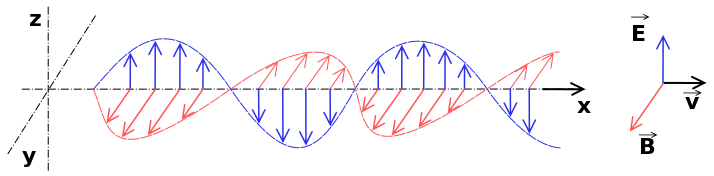
\includegraphics[width=.8\linewidth]{Figures/emf.png}
    \caption{Электромагнитная волна}
    \label{fig:emf}
\end{figure}

Радиоволны --- электромагнитное излучение с длинами волн в электромагнитном спектре длиннее инфракрасного света~\cite{wiki:radiowaves}. Радиоволны имеют частоту от 3 кГц до 300 ГГц, и соответствующую длину волны от 1 миллиметра до 100 километров. Естественными источниками радиоволн являются молнии и астрономические объекты. Искусственно созданные радиоволны используются для стационарной и мобильной радиосвязи, радиовещания, радиолокации и других навигационных систем, спутников связи, компьютерных сетей и других бесчисленных приложений. Различные частоты радиоволн по-разному распространяются в атмосфере Земли: длинные волны могут покрыть часть Земли очень последовательно, более короткие волны могут отражаться от ионосферы и распространяются по всему миру, и с еще более короткими длинами радиоволны изгибаются или отражаются очень слабо и распространяются в пределах прямой видимости.

Земная атмосфера прозрачна почти полностью для падающего извне излучения лишь в двух сравнительно узких окнах: оптическом --- в диапазоне длин волн $\lambda$ от 0.3 мкм до 2 мкм (область до 8 мкм состоит из ряда узких полос пропускания) и в радиодиапазоне --- для волн длиной от 1 мм до 30 м~\cite{astronet:atmosphere}. Непрозрачность атмосферы для всех др. длин волн определяется поглощением и рассеянием излучения на молекулах и атомах, а также отражением радиоволн от электронов ионосферы (рисунок~\ref{fig:atmosphere}~\cite{wiki:radiowaves}).

\begin{figure}[ht]
    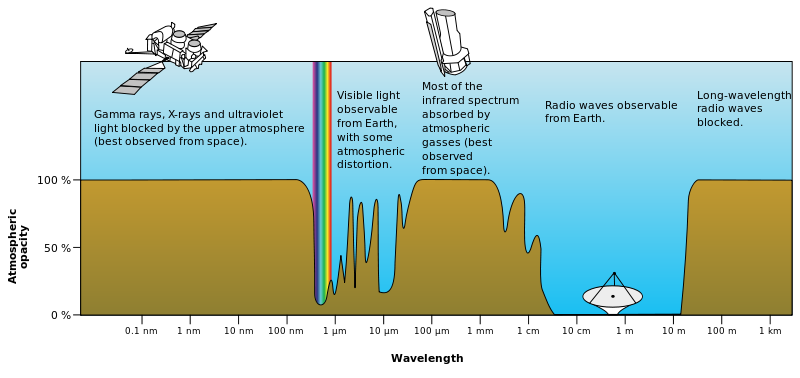
\includegraphics[width=1\linewidth]{Figures/radiowaves.png}
    \caption{Непрозначность атмосферы Земли для различных длин волн электромагнитного излучения, включая радиоволны}
    \label{fig:atmosphere}
\end{figure}

Электромагнитные волны (радиоволны) распространяются в вакууме со скоростью света --- 299, 792, 458 м/с.

Частота колебаний выражается через длину волны (формула~\eqref{eq:lambda}):

\begin{equation}
    \label{eq:lambda}
    f = \frac{c}{\lambda},
\end{equation}

где f --- частота, $\lambda$ --- длина волны, c --- скорость света.

Радиоволны подразделяются на несколько диапазонов (таблица~\ref{tab:radiorange}):

\begin{longtable}[c]{|c|c|c|}
    \caption{Диапазон радиоволн}
    \label{tab:radiorange}\\
    \hline
    \textbf{Диапазон} & \textbf{Частота} & \textbf{Длина волны}\\
    \hline
    \endfirsthead
    \hline
    \textbf{Диапазон} & \textbf{Частота} & \textbf{Длина волны}\\
    \hline
    \endhead
        Сверхдлинные <<СДВ>> & 3 -- 30 кГц & 100 -- 10 км\\
        \hline
        Длинные <<ДВ>> & 30 -- 300 кГц & 10 -- 1 км\\
        \hline
        Средние <<СВ>> & 300 -- 3000 кГц & 1000 -- 100 м\\
        \hline
        Короткие <<КВ>> & 3 -- 30 МГц & 100 -- 10 м\\
        \hline
        Ультракороткие <<УКВ>> & 30 МГц -- 6000 ГГц & 10 м -- 0.05 мм\\
        \hline
\end{longtable}

Ультракороткие, в свою очередь, включают (таблица~\ref{tab:ultrarange}):

\begin{longtable}[c]{|c|c|c|}
    \caption{Ультракороткие радиоволны}
    \label{tab:ultrarange}\\
    \hline
    \textbf{Диапазон} & \textbf{Частота} & \textbf{Длина волны}\\
    \hline
    \endfirsthead
    \hline
    \textbf{Диапазон} & \textbf{Частота} & \textbf{Длина волны}\\
    \hline
    \endhead
        Метровые <<МВ>> & 30 -- 300 МГц & 10 -- 1 м\\
        \hline
        Дециметровые <<ДМВ>> & 300 -- 3000 МГц & 10 -- 1 дм\\
        \hline
        Сантиметровые <<СМВ>> & 3 -- 30 ГГц & 10 -- 1 см\\
        \hline
        Миллиметровые <<ММВ>> & 30 -- 300 ГГц & 10 -- 1 мм\\
        \hline
        Субмиллиметровые <<СММВ>> & 300 -- 6000 ГГц & 1 -- 0.05 мм\\
        \hline
\end{longtable}

Диапазоны от дециметровых до миллиметровых волн, из-за их очень высокой частоты, называют сверхвысокими частотами <<СВЧ>>.

Распространение волны ограничивается её длиной: чем выше длина волны (меньше частота), тем она более способна огибать препятствия.


        \subsubsection{Передача информации радиоволнами}
        Для передачи информации радиоволну необходимо модулировать сигналом, содержащим информацию. Длинные, средние и короткие волны обычно имеют амплитудную модуляцию <<AM>>. Ультракороткие волны обычно имеют частотную модуляцию <<FM>>.

Модуляция (лат. modulatio --- размеренность, ритмичность) --- процесс изменения одного или нескольких параметров высокочастотного несущего колебания по закону низкочастотного информационного сигнала (сообщения)~\cite{wiki:modulation}.

Передаваемая информация заложена в управляющем (модулирующем) сигнале, а роль переносчика информации выполняет высокочастотное колебание, называемое несущим. Модуляция, таким образом, представляет собой процесс <<посадки>> информационного колебания на заведомо известную несущую.

В результате модуляции спектр низкочастотного управляющего сигнала переносится в область высоких частот. Это позволяет при организации вещания настроить функционирование всех приёмо-передающих устройств на разных частотах с тем, чтобы они <<не мешали>> друг другу.

Амплитудная модуляция представлена на рисунке~\ref{fig:am}. Этот тип модуляции изменяет \textbf{амплитуду} несущей частоты под действием кодирующего колебания (сигнала). Главный её недостаток --- низкая помехоустойчивость.

\begin{figure}[ht]
    \subfloat[]{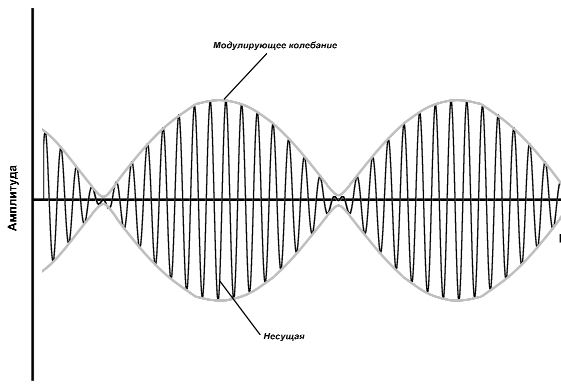
\includegraphics[width=.6\linewidth]{Figures/am.jpg}}
    \subfloat[]{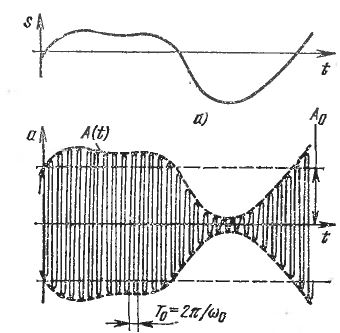
\includegraphics[width=.4\linewidth]{Figures/amclose.jpg}}
    \caption{Амплитудная модуляция (а) общая картина; (б) изменение несущего колебания по заданному закону}
    \label{fig:am}
\end{figure}

Частотная модуляция (рисунок~\ref{fig:fm}) --- изменение несущей \textbf{частоты} под воздействием кодирующего сигнала. Этот вид модуляции имеет более высокую помехоустойчивость несмотря на свою аналоговую природу.

\begin{figure}[ht]
    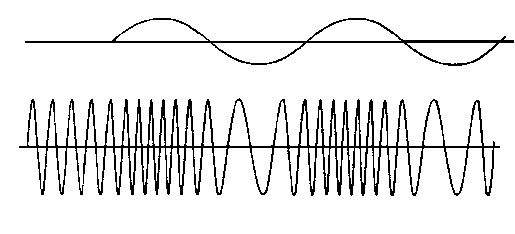
\includegraphics[width=.8\linewidth]{Figures/fm.jpg}
    \caption{Частотная модуляция}
    \label{fig:fm}
\end{figure}

Фазовая модуляция (рисунок~\ref{fig:pm}) --- изменение фазы несущей частоты скачкообразно (манипуляция). Недостаток данной модуляции в том, что ошибка в одном символе может привести к некорректному приёму всех последующих.

\begin{figure}[ht]
    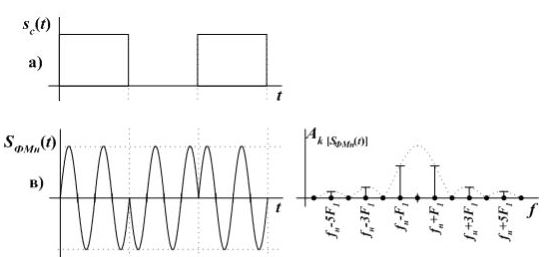
\includegraphics[width=.8\linewidth]{Figures/pm.jpg}
    \caption{Фазовая модуляция}
    \label{fig:pm}
\end{figure}

Дифференциально-фазовая манипуляция --- изменение фазы несущей частоты только при изменении разности (в данном случае --- при приходе каждой <<1>>).


        \subsubsection{Устройство радиопередатчика}
        Современный радиопередатчик состоит из следующих конструктивных частей (рисунок~\ref{fig:radiostruct})~\cite{wiki:radiotransmitter}:

\begin{itemize}
    \item задающий генератор частоты (фиксированной или перенастраиваемой) несущей волны;
    \item модулирующее устройство, изменяющее параметры излучаемой волны (амплитуду, частоту, фазу или несколько параметров одновременно) в соответствии с сигналом, который требуется передать (часто задающий генератор и модулятор выполняют в одном блоке — возбудитель);
    \item усилитель мощности, который увеличивает мощность сигнала возбудителя до требуемой за счёт внешнего источника энергии;
    \item устройство согласования, обеспечивающее максимально эффективную передачу мощности усилителя в антенну;
    \item антенна, обеспечивающая излучение сигнала.
\end{itemize}

\begin{figure}[ht]
    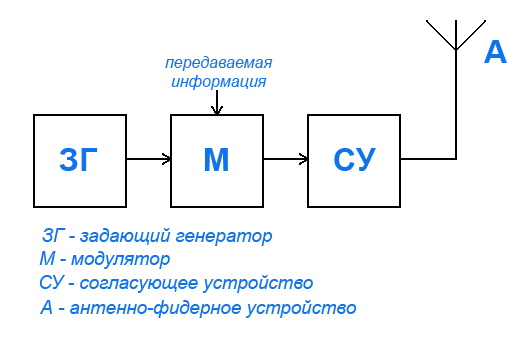
\includegraphics[width=.6\linewidth]{Figures/radiostruct.jpg}
    \caption{Структурная схема радиопередатчика}
    \label{fig:radiostruct}
\end{figure}

Принципиальная схема простейшего радиопередатчика представлена на рисунке~\ref{fig:rfcircuit}.

\begin{figure}[ht]
    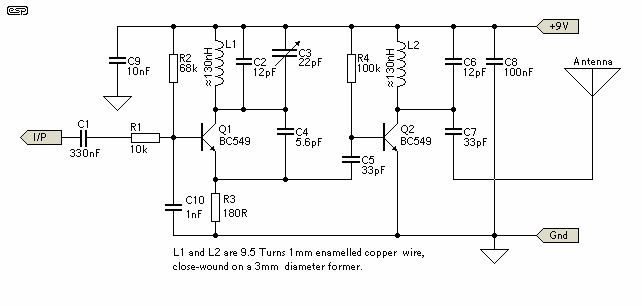
\includegraphics[width=1\linewidth]{Figures/rfcircuit.png}
    \caption{Простейшая принципиальная схема радиопередатчика}
    \label{fig:rfcircuit}
\end{figure}


        \subsubsection{Подбор антенны}
        Антенна --- устройство, преобразующее энергию высокочастотного колебания от передатчика в электромагнитную волну, способную распространяться в пространстве. Или в случае приёма --- производит обратное преобразование (электромагнитную волну в ВЧ колебания)~\cite{habr:antenna}.

Простейшая антенна --- симметричный вибратор: два токопроводящих отрезка, каждый из которых равен 1/4 длины волны (рисунок~\ref{fig:symvibr}). Широко применяется для приема телевизионных передач, как самостоятельно, так и в составе комбинированных антенн. Так, к примеру, если диапазон метровых волн телепередач проходит через отметку 200 МГц, то длина волны будет равна 1,5 м. Каждый отрезок симметричного вибратора будет равен 0,375 метра.

\begin{figure}[ht]
    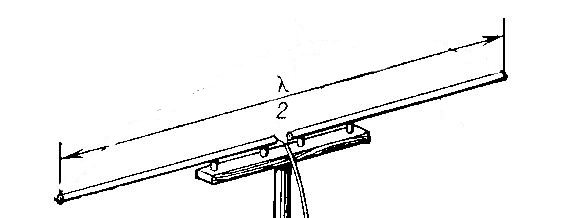
\includegraphics[width=.6\linewidth]{Figures/symvibr.jpg}
    \caption{Симметричный вибратор}
    \label{fig:symvibr}
\end{figure}

Несимметричный вибратор (штырьевая антенна) --- <<половина>> симметричного вибратора, установленного вертикально (рисунок~\ref{fig:asymvibr}). В качестве длины вибратора, применяют 1, 1/2 или 1/4 длины волны. Коэффициент направленного действия у несимметричного вибратора в два раза больше, чем у симметричного, за счет того, что вся мощность излучается в более узком направлении.

\begin{figure}[ht]
    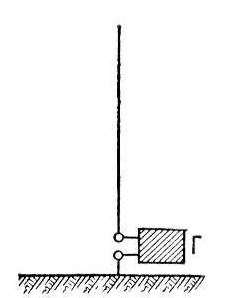
\includegraphics[width=.2\linewidth]{Figures/asymvibr.jpg}
    \caption{Несимметричный вибратор}
    \label{fig:asymvibr}
\end{figure}

При использовании приёмопередатчиков, работающих на частоте 433 МГц, длина волны $\lambda = 692$ мм. Соответственно, длина штырьевой антенны будет равна 69.2, 34.6 или 17.3 см.

Также существуют другие, более сложные типы антенн.

Поляризация --- это направленность вектора электрической составляющей электромагнитной волны в пространстве. Различают: вертикальную, горизонтальную и круговую поляризацию (рисунок~\ref{fig:polarization}).

\begin{figure}[ht]
    \subfloat[]{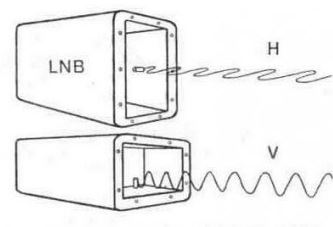
\includegraphics[width=.5\linewidth]{Figures/vgpolar.jpg}}
    \subfloat[]{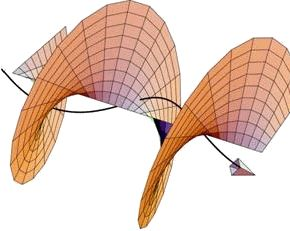
\includegraphics[width=.5\linewidth]{Figures/circlepolar.jpg}}
    \caption{Поляризация (а) горизонтальная и вертикальная; (б) круговая}
    \label{fig:polarization}
\end{figure}

Поляризация зависит от типа антенны и её расположения. К примеру, вертикально расположенный несимметричный вибратор, дает вертикальную поляризацию, а горизонтально расположенный --- горизонтальную.

Антенны горизонтальной поляризации дают больший эффект, т. к. природные и индустриальные помехи, имеют в основном вертикальную поляризацию. Горизонтально поляризованные волны, отражаются от препятствий менее интенсивно, чем вертикально. При распространении вертикально поляризованных волн, земная поверхность поглощает на 25\% меньше их энергии.


    \subsection{Принципы радиолокации}
    Радиолокацией называется обнаружение, определение координат и параметров движения различных объектов (целей), отражающих, переизлучающих или излучающих электромагнитную энергию (радиоволны). Термин <<локация>> происходит от латинского location – размещение, расположение. Комплекс радиотехнических устройств, выполняющих указанную задачу, представляет собой радиолокационную станцию (РЛС), или радиолокатор.

Радиолокация основана на следующих физических явлениях~\cite{wiki:radiolocation}:

\begin{enumerate}
    \item Радиоволны рассеиваются на встретившихся на пути их распространения электрических неоднородностях (объектами с другими электрическими свойствами, отличными от свойств среды распространения). При этом отражённая волна, также, как и собственно, излучение цели, позволяет обнаружить цель.
    \item На больших расстояниях от источника излучения можно считать, что радиоволны распространяются прямолинейно и с постоянной скоростью, благодаря чему имеется возможность измерять дальность и угловые координаты цели (Отклонения от этих правил, справедливых только в первом приближении, изучает специальная отрасль радиотехники --- Распространение радиоволн. В радиолокации эти отклонения приводят к ошибкам измерения).
    \item Частота принятого сигнала отличается от частоты излучаемых колебаний при взаимном перемещении точек приёма и излучения (эффект Доплера), что позволяет измерять радиальные скорости движения цели относительно РЛС.
    \item Пассивная радиолокация использует излучение электромагнитных волн наблюдаемыми объектами, это может быть тепловое излучение, свойственное всем объектам, активное излучение, создаваемое техническими средствами объекта, или побочное излучение, создаваемое любыми объектами с работающими электрическими устройствами.
\end{enumerate}

Основа радиолокации --- нахождение прямолинейного расстояния между объектами. Например, если найти расстояние от одного и того же объекта к двум различным <<искателям>>, можно будет аналитически рассчитать угол и относительно точное местоположение объекта.


        \subsubsection{Существующие методы радиолокации}
        Существует 5 основных методов определения расстояния при помощи радиоволн~\cite{radiofreq:tof}:

\begin{itemize}
    \item Time-Of-Arrival (TOA) и Time-Of-Flight (TOF);
    \item Time-Difference-Of-Arrival (TDOA);
    \item Received-Signal-Strength-Indication (RSSI);
    \item Near-Field-Electromagnetic-Ranging (NREF);
    \item Angle-Of-Arrival (AOA).
\end{itemize}

Метод TOA (TOF) заключается в измерении времени полёта сигнала, на основании которого рассчитывается расстояние.

RSSI в свою очередь измеряет угасание сигнала. Простота этого метода легла в основу широкого спектра устройств.

NREF измеряет сдвиг фазы между электрической и магнитной составляющей, работая на очень низких частотах (порядка 530 -- 1710 кГц).

TDOA использует набор синхроузлов как известные <<радиоточки>>. Гальваническая связь между <<точками>> обязательна для преодоления задержек. Из-за этого TDOA-решения достаточно комплексны и дороги, что ограничивает использование в спектре лишь специфичных архитектурных решений.

AOA использует сложные массивы антенн для измерения угла полученного сигнала. Из-за больших размеров таких массивов данное решение не подходит для компактных систем автоматизации <<радиометками>> в производственных цехах.

В основном, когда рассматривают метод TOF, зачастую сравнивают его с ближайшим <<родственником>> - RSSI. И RSSI, и TOF измеряют расстояние простой посылкой электромагнитного сигнала. Когда RSSI-метод определяет расстояние путём определения, на какую величину уровень сигнала упал по сравнению с исходным уровнем, TOF-метод определяет расстояние путём конкретной отправки сигнала в одну и другую сторону и измерением \textbf{времени} полёта радиоволны на заданном расстоянии.

Отсюда можно сделать очевидный вывод, что RSSI-устройства просты в исполнении, но обладают низкой точностью и интерферируют с подобными устройствами. Когда TOF-устройства достаточно точны, однако требуют высокой частоты работы для высокой точности на маленьких расстояниях.


        \subsubsection{Преимущества метода ToF}
        Уровень принимаемого сигнала не является надёжным параметром для локализации радиометок внутри помещения. На такое измерение влияет как погрешность во времени, так и факторы конкретной среды (помещения). Погрешность во времени возникает, в основном, из-за добавочного шума и интерференции и может быть значительно понижена за счет усреднения большого количества измерений. Факторы внешней среды --- непредсказуемы и являются случайными. В помещениях с большим количеством препятствий (сложные цеха, склады) измерение расстояния уровнем принимаемого сигнала является неточным.

Метод \textit{Time of Flight} более обещающий подход для измерения расстояния между двумя устройствами. Точное измерение времени должно дать точную оценку расстояния по сравнению с измерением, где используется лишь уровень сигнала. Однако, такой метод требует относительно быстрого и стабильного оборудования.

Благодаря тому, что радиоволны перемещаются со скоростью света и с лёгкостью огибают препятствия (на относительно низкой частоте), Time of Flight является идеальным методом для определения расстояния до объекта, находящегося в сложном помещении (цеха, склады). А измерение точного времени возврата определённого сигнала между двумя объектами позволяет избежать интерференции сигналов (как в случае RSSI).


\section{РЕАЛИЗАЦИЯ МЕТОДА TOF}
% Метод исследования (наблюдение, эксперимент, расчет, имитация).

    \subsection{Принцип метода ToF}
    Реализация метода \textit{Time of Flight} заключается в следующем: радиоволна летит от источника к приёмнику, который работает в режиме ретранслятора. Приёмник отправляет сигнал назад источнику, который фиксирует время полёта сигнала. Поделив это время на 2, получим время полёта сигнала от источника к приёмнику (формула~\eqref{eq:timeflight}):

\begin{equation}
    \label{eq:timeflight}
    t = \frac{T_f}{2},
\end{equation}

где $T_f$ --- время полёта (flight) от источника к приёмнику и обратно.

На рисунке~\ref{fig:tofscheme} представлена функциональная схема такого устройства.

\begin{figure}[ht]
    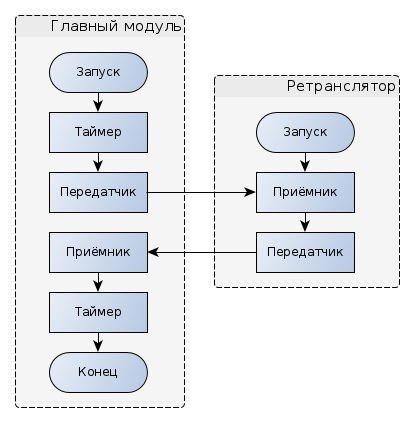
\includegraphics[width=.65\linewidth]{Figures/tofscheme.png}
    \caption{Функциональная схема устройства \textit{Time of Flight}}
    \label{fig:tofscheme}
\end{figure}

Электромагнитное излучение преодолевает расстояние со скоростью около 300.000.000 м/с. Таким образом, чтобы успеть <<словить>> время пролёта электромагнитной волны, детектор должен работать на частоте, равной или превышающей время пролёта сигнала от источника к приёмнику и обратно (формула~\eqref{eq:freqflight}). Чем более высокой будет частота работы устройства, тем больше будет его разрешающая способность и тем более точные результаты мы получим.

\begin{equation}
    \label{eq:freqflight}
    f = \frac{1}{T_f} = \frac{c}{S},
\end{equation}

где c --- скорость света, S --- минимально возможное расстояние, на котором прибор с данной частотой должен успевать уловить время $T_f$ полёта радиоволны.

Таким образом, для обеспечения работы на расстоянии в 3 метра, устройство должно работать на частоте как минимум $f = \frac{300.000.000}{3} = 100$ МГц. Для 300 метров --- 1 МГц.

Для уменьшения необходимой частоты работы устройства, а также сокращению возможных погрешностей и ошибок, воспользуемся методом <<накопления>> ToF.

    % Разработка структурной и принципиальной схемы.
    % Почему мы используем именно ToF.

    \subsection{Принцип метода <<накопления>> ToF}
    \label{sec:accumulation}
    Метод <<накопления>> ToF заключается в следующем: устройство с заведомо более низкой частотой, чем необходимо, неспособное уловить время $T_f$ на заданном расстоянии, производит ту же последовательность действий (посылает сигнал ретранслятору и принимает его назад), но не останавливается, а продолжает посылать и принимать сигнал N-ное количество раз. Через заданный интервал времени (или через заданное число N итераций) устройство останавливается и определяет <<накопленное>> суммарное <<добавочное>> время. Это время, с определённой погрешностью, и будет временем $T_f \cdot N$ полёта, умноженным на N (рисунок~\ref{fig:accscheme}).

\begin{figure}[ht]
    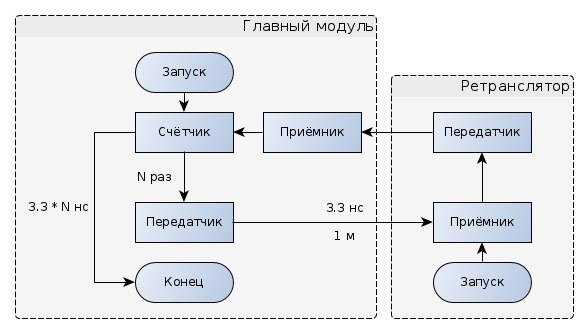
\includegraphics[width=1\linewidth]{Figures/accscheme.png}
    \caption{Функциональная схема метода <<накопления>> ToF}
    \label{fig:accscheme}
\end{figure}

Однако у данного метода есть и недостатки: чем ниже частота, тем больше будет время накопления результата. Для примера, возьмём частоту 1 Гц и расстояние 1 м. Тогда передатчик будет посылать данные приёмнику, ждать возврата сообщения, затем ждать секунду и посылать очередной пакет приёмнику.

На расстоянии 1 м. время полёта пакета от источника к приёмнику будет равно $T_f = \frac{1}{300.000.000} = 3.3$ нс.

Как будет сказано ниже, разрешение (погрешность) микроконтроллеров ATmega (Arduino) составляет около 4-10 мксек. В данном примере, возьмём 50 мксек для надёжности. Время, необходимое для того, чтобы микроконтроллер зарегистрировал изменение, будет равно:

\begin{equation}
t_w = \frac{\Delta\tau}{T_f} = \frac{50 \cdot 10^{-6}~\textrm{с}}{3.3 \cdot 10^{-9}~\textrm{с}} = 15151~\textrm{с} = 252~\textrm{мин} = 4.2~\textrm{ч}
\end{equation}

Обычно на практике применяются расстояния больше 1 метра, что сокращает время ожидания результата пропорционально расстоянию. Задача сводится к увеличению частоты работы устройства.


    \subsection{Препятствия реализации метода <<накопления>> ToF}
    При передаче радиоволны с одного устройства на другое, замеренное время будет кратно тактовой частоте устройства, что ограничивает применение метода <<накопления>>. Время выполнения одного такта \textbf{работы} устройства должно быть равно или меньше времени полёта волны от одного устройства к другому. Например, если время полёта волны будет 3.3 нс, а такт процессора устройства будет занимать 33.3 нс, мы получим погрешность (задержку) в 10 раз больше чем само время Time of Flight. И т. к. время TOF будет <<ожидать>> следующий такт процессора чтобы <<быть отмеченным>>, мы получим данные с погрешностью горзадо более большой (в 10 раз больше) чем мы могли бы ожидать. Для частоты работы Arduino (16 МГц) мы получим дискретизацию в 20 метров независимо от того, какие приёмопередатчики мы будем использовать и на каком расстоянии будем измерять TOF.


\section{АНАЛИЗ ПОМЕХ TOF-ИЗМЕРЕНИЯ}
% Теория из иностранных источников.
% Ссылки на экспериментальные данные ниже.

    \subsection{Источники погрешностей метода ToF}
    \label{sec:error}
    Измерение расстояния методом \textit{Time of Flight} ограничено такими факторами, как синхронизация во времени, шумы, погрешности выборки и эффект многолучевого распространения. Этот раздел обобщает информацию о каждой возможной причине.

\subsubsection{Синхронизация во времени}

\textit{Time of Flight} системе необходимо измерить время между отправкой и принятием сигнала, используя общий отсчёт времени. В простейшем случае, устройство Б определяет удалённость от устройства А измеряя время прибытия сигнала от устройства А. Если "часы" синхронизированы не идеально (рисунок~\ref{fig:sync}), т. е. начало отсчёта t = 0 устройства Б содержит некоторое смещение относительно нуля устройства А, это добавляет дополнительную ошибку в измерение. Необходимая дискретизация синхронизации времени (1 нс = 30 см) зачастую слишком точная для многих систем~\cite{tof:lowcost}.

\begin{figure}[ht]
    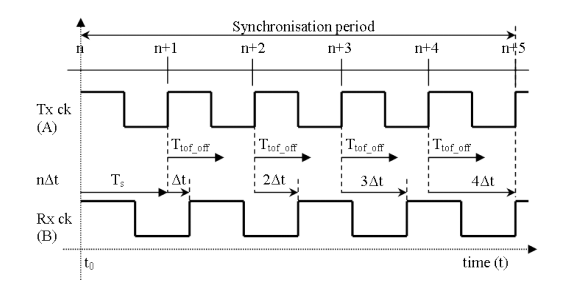
\includegraphics[width=.8\linewidth]{Figures/sync.png}
    \caption{Рассинхронизация частот двух тактовых генераторов}
    \label{fig:sync}
\end{figure}

Рассинхронизацию часов можно устранить при помощи метода <<Two Way Time Transfer>>, про который будет рассказано в главе~\ref{sec:mitigation} <<\nameref{sec:mitigation}>>.

\subsubsection{Шум}

Точность измерения расстояния в идеальном случае ограничего лишь белым шумом --- отношением <<энергия/шум>>, $E_S/N_0$ на приёмнике и используемой шириной частоты (bandwidth), $B$. Измерение дальности --- вопрос, изучаемый в контексте радаров, и неравенство Крамера-Рао обеспечивает нахождение нижней границы дисперсии оценки диапазона белого шума. Для односторонней системы нахождения расстояния используя IEEE 802.15.4 модуляцию, неравенство Крамера-Рао выглядит так (формула~\eqref{eq:crb}):

\begin{equation}
    \label{eq:crb}
    \sigma_r^2 >= \frac{c^2}{\frac{4 \pi^2 B^2 E_S}{N_0}},
\end{equation}

где $\sigma_r^2$ --- дисперсия оценки диапазона,
$c$ --- скорость света,
и $B$ --- используемая ширина полосы сигнала в Герцах.

Отношением <<сигнал/шум>> здесь является (формула~\eqref{eq:snr}):

\begin{equation}
    \label{eq:snr}
    \frac{E_S}{N_0} = t_S B \cdot SNR,
\end{equation}

где $t_S$ --- длительность сигнала, на время которого ширина полосы занята.

В большинстве сигналов, ширина полосы и длительность завязаны таким образом, что $t_S B \approx 1$. Таким образом, соотношение $\frac{E_S}{N_0}$ приблизительно равно SNR (отношению <<сигнал/шум>>).

Сигналы с $t_S B > 1$ будут проявлять лучшее шумоподавление за счет более низкого соотношения <<сигнал/шум>>, и таких сигналы называются <<pulse-compressed waveforms>>.

%\subsubsection{Погрешности выборки}

%Здесь про выборку.

%\subsubsection{Multipath channel effect}

%Здесь про многолучевое распространение.

    
    \subsection{Методы уменьшения погрешностей измерения ToF}
    \label{sec:mitigation}
    Уменьшения ошибки измерения можно добиться, в основном, следующими методами:

\begin{enumerate}
    \item Two Way Time Transfer.
    \item Code Modulus Synchronization.
    \item Frequency Diverse Range Estimation.
\end{enumerate}

\subsubsection{Two Way Time Transfer}

Метод <<Two Way Time Transfer>> (TWTT) --- метод, позволяющий устранить рассогласование начала отсчёта тактовой частоты двух устройств. Этот метод позволяет игнорировать смещение начала отсчёта первого устройства по отношению ко второму $\delta t$. Алгоритм работы TWTT показан на рисунке~\ref{fig:twttmethod}.

\begin{figure}[ht]
    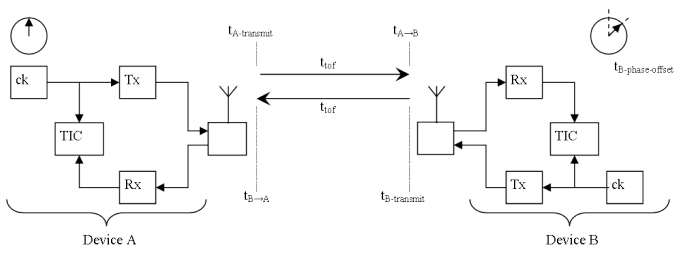
\includegraphics[width=1\linewidth]{Figures/twttmethod.png}
    \caption{Алгоритм работы метода Two-way Time Transfer}
    \label{fig:twttmethod}
\end{figure}

Метод заключается в следующем: оба устройства (А и Б) участвуют в измерении времени используя локальный (собственный) тактовый генератор. Если устройство А отправляет посылку в момент времени $t_{sA}$, устройство Б принимает посылку в момент времени $t_{rB}$, устройство Б отправляет посылку в момент времени $t_{sB}$ и устройство А принимает посылку в момент времени $t_{rA}$, причём $t_{sA} < t_{rB} < t_{sB} < t_{rA}$, тогда устройство A измерит время $t_A = t_{rA} - t_{sA}$, а устройство Б измерит время $t_B = t_{sB} - t_{rB}$. \textit{Time of Flight}, TOF, $\tau$ может быть выражена используя эти два времени следующим образом (формула~\eqref{eq:twtt}):

\begin{equation}
    \label{eq:twtt}
    \tau = \frac{t_A - t_B}{2}.
\end{equation}

В общем случае, можно представить метод Two-way Time Transfer следующими выражениями~\cite{tof:ranging}:

\begin{equation}
    t_{A \to B} = t_{A - transmit} + t_{TOF} + t_{B - offset}
\end{equation}

\begin{equation}
    t_{B \to A} = t_{B - transmit} + t_{TOF} - t_{B - offset}
\end{equation}

Тогда,

\begin{equation}
    t_{TOF} = \frac{1}{2}[(t_{A \to B} + t_{B \to A}) - (t_{A - transmit} + t_{B - transmit})]
\end{equation}

\begin{equation}
    t_{offset} = \frac{1}{2}[(t_{A \to B} - t_{B \to A}) - (t_{A - transmit} - t_{B - transmit})]
\end{equation}

%\subsubsection{Code Modulus Synchronization}

%Empty.

%\subsubsection{Frequency Diverse Range Estimation}

%Empty.


    \subsection{Расчёты и экспериментальные данные}
    \label{sec:error}
    Нижнюю границу диапазона ошибки TOF-метода абстрактно можно вычислить, используя вариант неравенства Крамера-Рао~\cite{radiofreq:tof}, представленный в формуле~\eqref{eq:cramer} (рисунок~\ref{fig:cramer}):

\begin{equation}
    \label{eq:cramer}
    \sigma^2_{TOF} >= \frac{1}{8\pi^2 \cdot \beta^2_f \cdot SNR \cdot n},
\end{equation}

где $\sigma^2_{TOF}$ --- дисперсия (ошибка TOF), $\beta_f$ --- спектральная ширина полученного сигнала в герцах, n --- число усреднённых TOF-измерений, SNR --- энергия на бит делённая на мощность шума ($E_b/N_0$).

\begin{figure}[ht]
    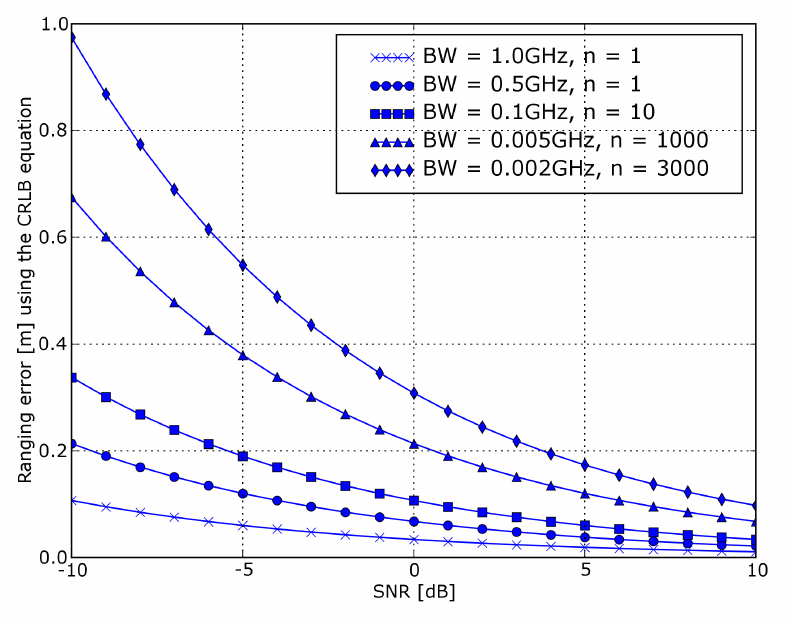
\includegraphics[width=.7\linewidth]{Figures/cramer.png}
    \caption{Нижняя граница диапазона TOF-ошибки}
    \label{fig:cramer}
\end{figure}

Из формулы~\eqref{eq:cramer} видно, что точность TOF-измерения квадратично растёт с увеличением спектральной ширины сигнала, из чего следует эффективность использования сверхширокой полосы. Всвязи с этим, делается вывод о невыгодности использования свободных 433-МГц несущих частот для передачи радиосигнала.


\section{ПОДБОР ОБОРУДОВАНИЯ}
% Технические средства исследования (установка, аппаратура, датчики, ВТ).

    \subsection{Микроконтроллеры}
    \label{sec:microcontroller}
    Микроконтроллер (англ. \textit{Micro Controller Unit, MCU}) --- микросхема, предназначенная для управления электронными устройствами \cite{wiki:microcontroller}. Типичный микроконтроллер сочетает на одном кристалле функции процессора и периферийных устройств, содержит ОЗУ и (или) ПЗУ. По сути, это однокристальный компьютер, способный выполнять относительно простые задачи. Микроконтроллер общается с внешним миром считывая значения на своих <<входах>> и выдавая соответствующие значения на своих <<выходах>>.

Общая структурная схема микроконтроллера представлена на рисунке~\ref{fig:microstruct}.

\begin{figure}[ht]
    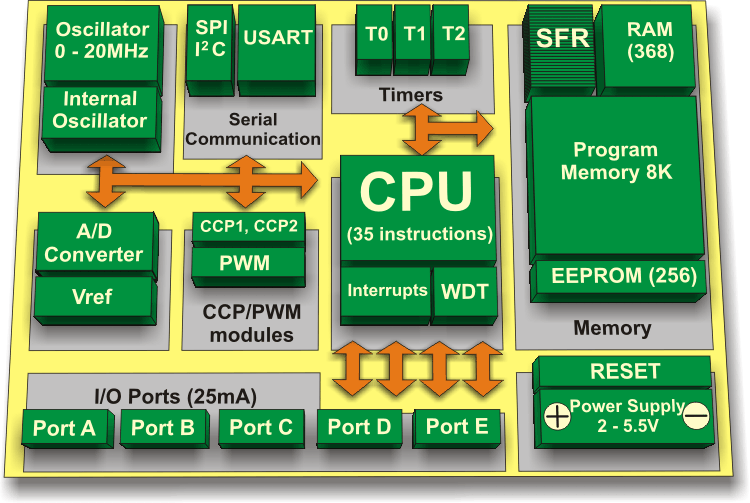
\includegraphics[width=.7\linewidth]{Figures/microstruct.png}
    \caption{Обобщённая структурная схема микроконтроллера}
    \label{fig:microstruct}
\end{figure}

Здесь можно наблюдать:

\begin{itemize}
    \item генератор задающей частоты (clock);
    \item последовательный UART-порт коммуникации с другими устройствами (например, по протоколу modbus);
    \item низкоуровневые таймеры (работающие на частотах начиная от задающей частоты и ниже);
    \item процессор с поддержкой прерываний;
    \item модуль широтно-импульсной модуляции;
    \item ЦАП/АЦП;
    \item порты ввода-вывода (аналоговые и цифровые);
    \item блок оперативной (RAM) и постоянной (EEPROM) запоминающей памяти.
\end{itemize}

Зачастую, частота работы микроконтроллеров недостаточна для обеспечения необходимой разрешающей способности Time of Flight устройства, и прибегают к \textbf{микропроцессорным} средствам, например платам на ARM-процессорах. Однако для целей моделирования был взят микроконтроллер ATMega, а точнее --- плата разработки Arduino, использующая в своём ядре микроконтроллер ATMega.

    % Больше деталей про ОЗУ, ПЗУ и другие части микроконтроллера (микропроцессора).

        \subsubsection{Характеристики и устройство atmega (328)}
        Фирма ATMEL --- один из лидеров производства микроконтроллеров. Микроконтроллеры ATmega в большинстве своём работают на частоте 16 МГц. Это означает, что одна инструкция программы выполняется за 1/16000000 секунды, т. е. выполняется 16 миллионов инструкций за 1 секунду. Блок-схема ATmega328 показана на рисунке~\ref{fig:atmegablock}~\cite{atmega:328}.

\begin{figure}[ht]
    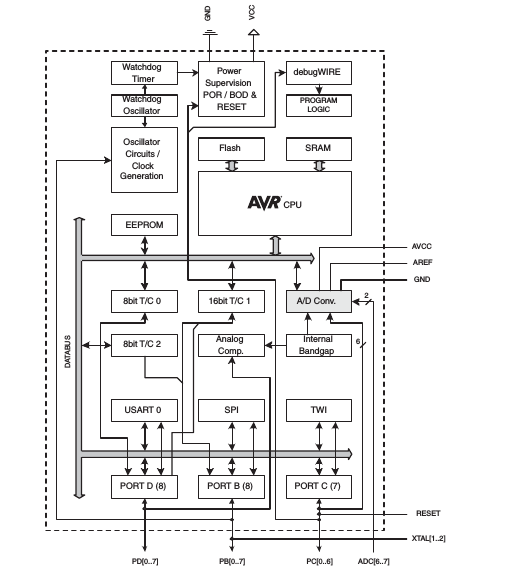
\includegraphics[width=.6\linewidth]{Figures/atmegablock.png}
    \caption{Блок-схема ATmega328}
    \label{fig:atmegablock}
\end{figure}


        \subsubsection{Аппаратно-программная среда arduino}
        Arduino --- аппаратно-программная платформа <<надстройки>> над микроконтроллерами ATmega, позволяющая быстро и удобно конструировать прототип устройства без необходимости подавать внешнее питание и позволяющая разрабатывать безпаечные макеты.

Arduino представляет собой плату, построенную вокруг ATmega, поддерживающую высокоуровневые инструкции на языке C++, а также предоставляющую удобный интерфейс для программирования через USB-интерфейс. Благодаря большому сообществу и наличию разных библиотек, разработка конечныйх устройств на Arduino представляет собой удобный и быстрый процесс по сравнению с работой непосредственно с микроконтроллером.

Схематика Arduino UNO представлена в приложении A.

Технические характеристики Arduino UNO и Arduino MEGA представлены в таблице~\ref{tab:megatech}~\cite{arduino:mega, arduino:uno}.

\begin{longtable}[c]{|p{2in}|c|c|}
    \caption{Технические характеристики Arduino UNO и Arduino MEGA}
    \label{tab:megatech}\\
    \hline
    \textbf{Параметр} & \textbf{UNO} & \textbf{MEGA}\\
    \hline
    \endfirsthead
    \hline
    \textbf{Параметр} & \textbf{UNO} & \textbf{MEGA}\\
    \hline
    \endhead
        Микроконтроллер & ATmega328 & ATmega2560\\
        \hline
        Оперируемое напряжение & \multicolumn{2}{c|}{5 В}\\
        \hline
        Входное напряжение (реккомендуемое) & \multicolumn{2}{c|}{7 -- 12 В}\\
        \hline
        Входное напряжение (максимальное) & \multicolumn{2}{c|}{6 -- 20 В}\\
        \hline
        Цифровые входы/выходы & 14 (~6) & 54 (~14)\\
        \hline
        Аналоговые входы & 6 & 16\\
        \hline
        Постоянные ток на 1 вход/выход & \multicolumn{2}{c|}{40 мА}\\
        \hline
        Постоянный ток на вход 3.3 В & \multicolumn{2}{c|}{50 мА}\\
        \hline
        Память & 32 Кб & 256 Кб\\
        \hline
        Частота задающего генератора & \multicolumn{2}{c|}{16 МГц}\\
        \hline
\end{longtable}

Условные обозначения элементов на плате Arduino показаны на рисунке~\ref{fig:specuno}.

\begin{figure}[ht]
    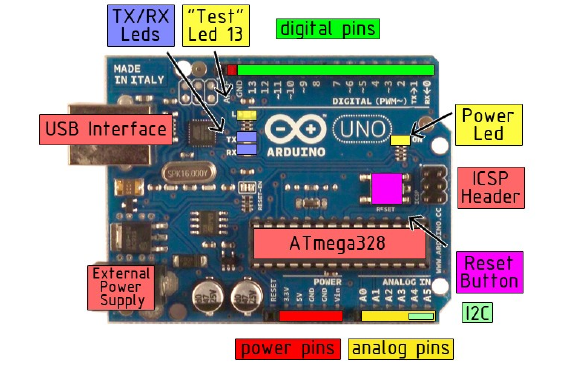
\includegraphics[width=.8\linewidth]{Figures/specuno.png}
    \caption{Спецификация Arduino UNO}
    \label{fig:specuno}
\end{figure}


    \subsection{Микропроцессоры}
    Как было показано в главах~\ref{sec:taskfreq} и~\ref{sec:error}, чем ниже частота работы конечного устройства, тем больше будет квадратичная ошибка измерения. Для целей Time of Flight измерения будут больше подходить микропроцессорные устройства с большей тактовой частотой, использующие датчики на частотах 2.4 ГГц (Wi-Fi). Частота 2.4 ГГц является открытой частотой, также как и 433 МГц. Однако возникает проблема интерференции с другими устройствами, т. к. большинство устройств в современном мире работают на частотах 2.4 ГГц и будут вмешиваться в сигнал разрабатываемого Time of Flight устройства. Также стоимость микропроцессорных высокочастотных устройств зачастую превышает стоимость микроконтроллеров.

В разработанной модели использовались микроконтроллеры в связи с наличием и простоте использования, однако при разработке конечного устройства будет целесообразнее использовать микропроцессорное устройство.

    % RaspberryPI, немного теории и экспериментальных данных. Аргументы за и против (цена).

    \subsection{Разработка физической модели}
    % Функциональная схема и её описание.
    % Электрическая принципиальная схема в деталях.
    % Выбор каждой детальки (подбор используемого, подбор необходимого).
    % Каждая деталька должна быть подробно описана.

        \subsubsection{Общая схема устройства}
        Общая блок-схема устройства представлена на рисунке~\ref{fig:commonscheme}.

\begin{figure}[ht]
    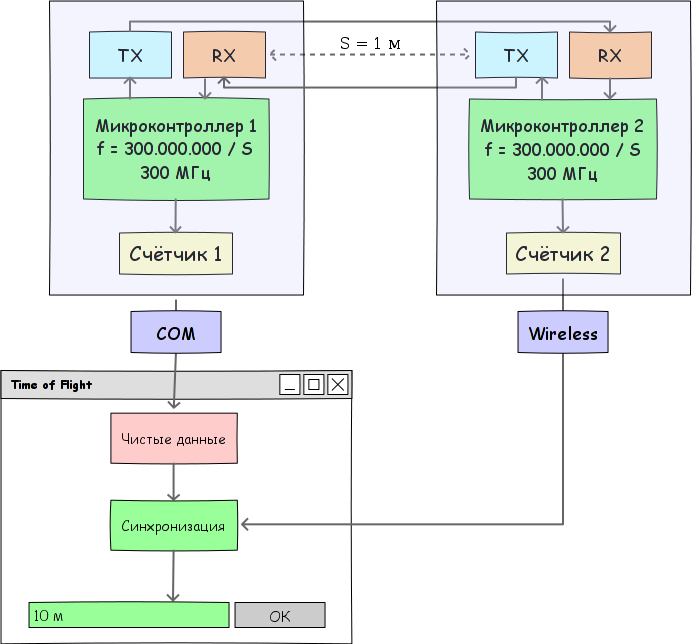
\includegraphics[width=1\linewidth]{Figures/commonscheme.png}
    \caption{Общая блок-схема Time of Flight устройства}
    \label{fig:commonscheme}
\end{figure}

Здесь модуль 1 соединён с ЭВМ посредством COM-порта, когда модуль 2 общается с модулем 1 лишь посредством радиосвязи. После завершения рассчёта времени Time of Flight, модуль 2 посылает данные, измеренные с помощью локального тактового генератора, на модуль 1 посредством радиосвязи, после чего модуль 1, пользуясь <<полной картиной>>, посылает данные на ЭВМ через последовательный порт.

Скорость общения по COM-порту была выбрана в 115200 бит/c.

Схема подключения оборудования одного модуля представлена на рисунке~\ref{fig:circscheme}.

\begin{figure}[ht]
    \subfloat[]{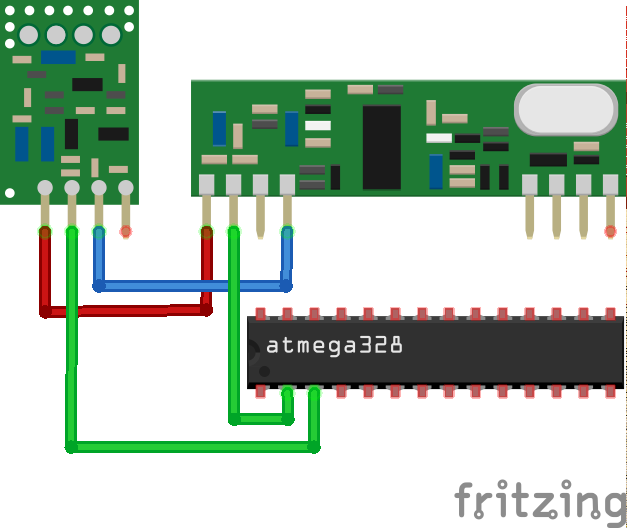
\includegraphics[width=.3\linewidth]{Figures/hardscheme.png}}
    \qquad
    \subfloat[]{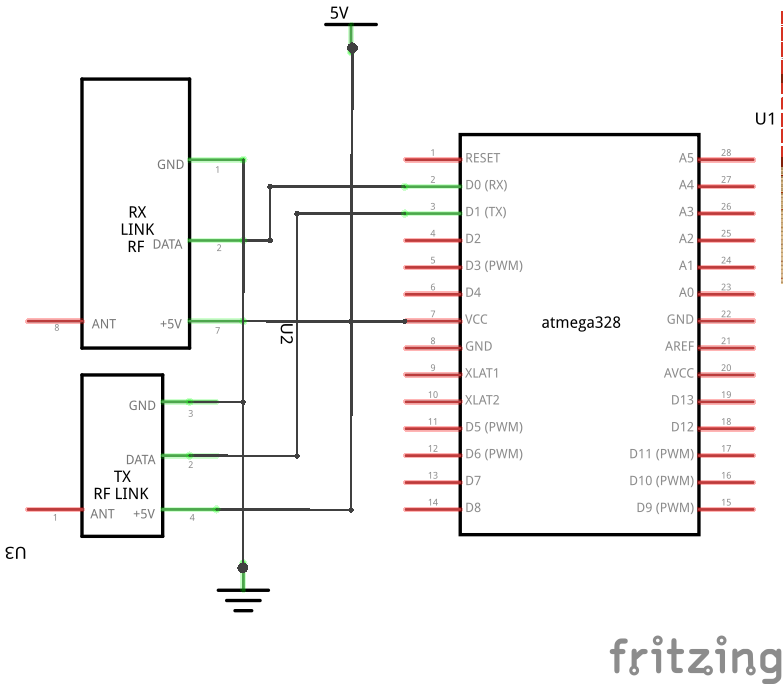
\includegraphics[width=.6\linewidth]{Figures/circscheme.png}}
    \caption{Подключение оборудования (а) общий вид; (б) схемотехника}
    \label{fig:circscheme}
\end{figure}

Здесь к микроконтроллерному модулю подключены передатчик и приёмник, работающие на несущей частоте 433 МГц и общающиеся непосредственно с другим модулем. Схема другого модуля будет выглядеть точно также, отличаться будет лишь исходный код программы.


        \subsubsection{Алгоритм работы устройства}
        Алгоритм работы программной части был представлен в главе~\ref{sec:coding} <<\nameref{sec:coding}>>.

В этой главе представлен набор сигналов, появляющихся на входах и выходах микроконтоллера с учётом подключенного оборудования. Алгоритм работы представлен на рисунке~\ref{fig:physalg}.

\begin{figure}[ht]
    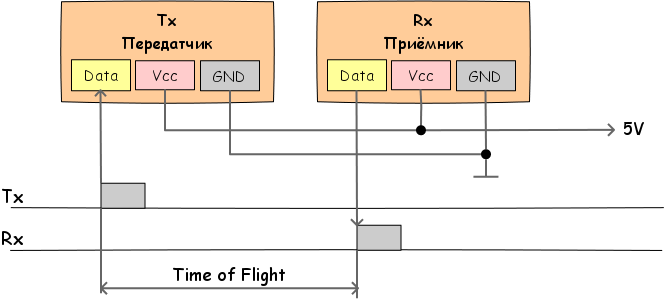
\includegraphics[width=.8\linewidth]{Figures/physalg.png}
    \caption{Алгоритм работы устройства}
    \label{fig:physalg}
\end{figure}


\section{РАЗРАБОТКА ПРОГРАММНОЙ МОДЕЛИ}
\label{sec:coding}
В процессе разработки программного обеспечения был создан универсальный модуль общения ЭВМ с устройством (микроконтроллером) посредством последовательного COM-интерфейса, поддерживающий внедрение во встраиваемые системы, например --- SCADA-системы.

Модуль расчёта расстояния (программа микроконтроллера) также является модульной: каждое устройство представляет собой законченный модуль, который можно перевести в режим сервера опроса из стандартного режима <<радиометки>>.

При написании исходного кода программ, были использованы наиболее популярные в сфере автоматизации технологии для избежания конфликтов внедрения в существующие SCADA-системы.

% Методика исследования (этапы, план, ПО, математический аппарат).
% Исходный код arduino и C# с описанием блоков и алгоритмом работы.
% Отдельная DLL для встраиваемых SCADA-систем.

    \subsection{Выбор программной среды}
    При разработке программы для программно-аппаратной системы Arduino была использована IDE Arduino 1.6.4 как наиболее простой вариант для компиляции и прошивки программы в память микроконтроллера. IDE Arduino представляет собой свободное программное обеспечение для разработки управляющих программ платформы Arduino.

При разработке программного модуля общения ToF-устройства с ЭВМ, была использована Microsoft Visual Studio 2013 Community --- свободная среда разработки от корпорации Microsoft с возможностью разработки на многих языках, включая Arduino, а также под многие платформы, включая .NET и Android.

Функциональная схема обоих программных модулей представлена на рисунке~\ref{fig:softwarefunc}.

\begin{figure}[ht]
    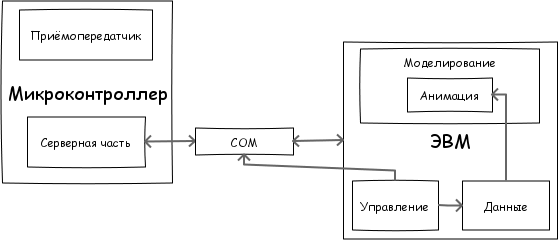
\includegraphics[width=.8\linewidth]{Figures/softwarefunc.png}
    \caption{Функциональная схема программных модулей}
    \label{fig:softwarefunc}
\end{figure}


    \subsection{Выбор языка программирования}
    Разработка управляющей программы осуществляется на языке СИ для совместимости с большинством микроконтоллеров. Для целей моделирования, программа была разработана на диалекте языка СИ <<Arduino>>, специально созданном для аппаратно-программной платформы <<Arduino>>.


    \subsection{Разработка программной модели}
    
        \subsubsection{Алгоритм работы}
        Алгоритм работы программы представлена на рисунке~\ref{fig:codeblock}.

\begin{figure}[ht]
    \subfloat[]{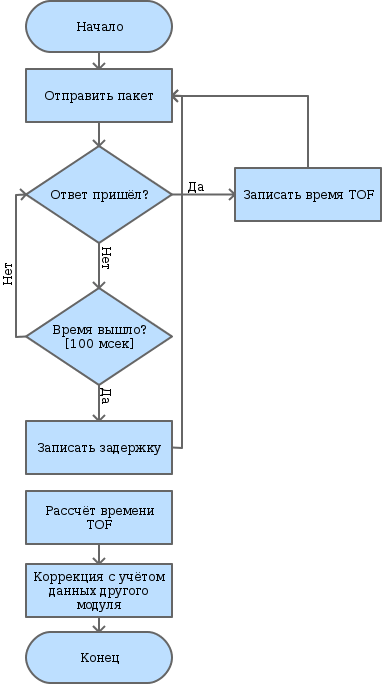
\includegraphics[width=.5\linewidth]{Figures/codeblock.png}}
    \qquad
    \subfloat[]{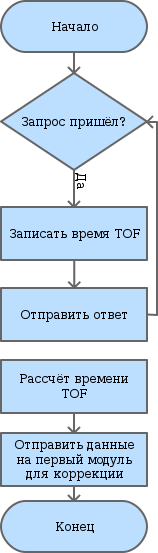
\includegraphics[width=.2\linewidth]{Figures/codeblock2.png}}
    \caption{Алгоритм программной модели (а) модуля-сервера; (б) модуля-клиента (радиометки)}
    \label{fig:codeblock}
\end{figure}


        \subsubsection{Библиотека передачи данных}
        Для средств моделирования устройства выбирается библиотека VirtualWire, однако стоит рассмотреть вариант создания собственной, более быстрой библиотеки для общения между двумя микропроцессорными модулями.

На радиопринимающей стороне необходимо отфильтровать актуальные данные от постоянно находящихся на ней шумов, т. е. необходимо <<сконструировать>> программный детектор, способный принять пакет данных. Для этого необходимо разработать специфичный протокол передачи данных, где сообщению будет предшествовать некая <<шапка>>, состоящая из определённого количества бит. Эта шапка будет детектироваться приёмником, и всё что идёт после неё будет считаться сообщением (определённой длины). Для увеличения надёжности посылки, имеет смысл продублировать сообщение в обратном порядке, или же воспользоваться другими существующими алгоритмами повышения надёжности передачи (например, Cyclic Redundancy Check CRC-16).


        \subsubsection{Модуль приёмопередатчика}
        Программа модуля на arduino представляет собой постоянно выполняющийся цикл в функции \textbf{loop()}. По умолчанию программа работает в режиме ретранслятора (клиента): пришедшее на приёмник сообщение отправляется назад и включается таймер времени для расчёта, используя локальные часы (Two Way Time Transfer, глава~\ref{sec:mitigation}). Если сообщение на приёмник не приходит, работа устройства не начинается. При подключении модуля к ПК, можно перевести его в режим сервера: контроллер будет сначала посылать сообщение, а затем рассчитывать время, которое радиоволна летит в пространстве. Также в режиме сервера устройство посылает следующее сообщение при невозможности получить ответ за определённое время (таймаут).

\begin{minted}[gobble=4,fontsize=\footnotesize]{c}
    #include <VirtualWire.h>
    int tx = 1; // Вход приёмника.
    int rx = 0; // Выход передатчика.
    bool server = false; // Переключатель режима сервера.
    const char *txMessage = "1"; // Сообщение для передачи.
    const char *rxMessage = "0"; // Сообщение для получения.
    uint8_t buf[VW_MAX_MESSAGE_LEN];
    uint8_t buflen = VW_MAX_MESSAGE_LEN;
    int timeout = 300;

    void setup()
    {
        Serial.begin(115200); // Общение с ПК.
        vw_set_tx_pin(tx);
        vw_set_rx_pin(rx);
        vw_set_ptt_inverted(true);
        vw_setup(9600); // Скорость передачи.
        vw_rx_start();
    }

    void loop()
    {
        if (Serial.available() > 0)
        if (Serial.read() == 's')
            server = true; // Установить режим сервера.
        else
            server = false; // Установить режим клиента.

        if (server)
            vw_send((uint8_t *)txMessage, strlen(txMessage));
        int sendTime = micros();

        vw_wait_rx_max(300);
        if (vw_get_message(buf, &buflen))
        {
            int tof = micros() - sendTime;
            if (!server)
                vw_send((uint8_t *)rxMessage, strlen(rxMessage));
        }
    }
\end{minted}

Учитывая ограничения VirtualWire (как будет показано в главе~\ref{sec:virtualwirefreq}), а также ограничения используемых датчиков (глава~\ref{sec:fs1000a}), построить работающий прототип с её использованием не представляется возможным. Библиотека VirtualWire была использована для \textbf{моделирования} части, отвечающей за беспроводную передачу пакета и рассчёт времени Time of Flight.


        \subsubsection{Модуль управления для ЭВМ}
        Модуль управления представляет собой динамическую библиотеку (dll) с набором методов и внешним API, способную встраиваться в любую SCADA- или другую систему. В процессе создания решения был написан стандартный графический интерфейс для удобного моделирования разных частей проекта, использующий dll-библиотеку.

Встраиваемая библиотека имеет следующие функции:

\begin{itemize}
    \item включение и отключение режима <<сервер>>;
    \item вывод расчитанного расстояния между сервером и клиентом (на экран).
\end{itemize}

Исходный код DLL-модуля представлен ниже:

\begin{minted}[gobble=4,fontsize=\footnotesize]{csharp}
    using System.IO.Ports;

    namespace TOF
    {
        public class TOF
        {
            public static string GetFirstPort()
            {
                try
                {
                    return SerialPort.GetPortNames()[0];
                }
                catch { return ""; }
            }

            private SerialPort sp;
            private bool server = false;
            public bool ServerMode
            {
                get { return server; }
                set
                {
                    try
                    {
                        server = ServerMode;
                        if (server)
                            sp.Write("s");
                        else
                            sp.Write("c");
                    }
                    catch { }
                }
            }
            public TOF(string portName = "COM1")
            {
                try
                {
                    sp = new SerialPort(portName, 115200);
                    sp.Open();
                }
                catch { }
            }

            public string Read()
            {
                try
                {
                    if (sp.BytesToRead != 0)
                        return sp.ReadExisting();
                    else
                        return "";
                }
                catch { return ""; }
            }
        }
    }
\end{minted}

Программа управления процессом моделирования имеет следующие возможности:

\begin{itemize}
    \item отображение анимации передачи и приёма пакета;
    \item отображение информации последовательного COM-порта;
    \item управляющие функции (функции встраиваемой библиотеки).
\end{itemize}

Исходный код программы управления представлен ниже:

\begin{minted}[gobble=4,fontsize=\footnotesize,breaklines=true]{csharp}
    // Program.cs

    using System;
    using System.Windows.Forms;

    namespace TimeOfFlight
    {
        static class Program
        {
            [STAThread]
            static void Main()
            {
                Application.EnableVisualStyles();
                Application.Run(new MainForm());
            }
        }
    }

    // MainForm.cs
    using System;
    using System.Windows.Forms;

    namespace TimeOfFlight
    {
        public partial class MainForm : Form
        {
            TOF.TOF tof;

            public MainForm()
            {
                InitializeComponent();
                inputPort.Text = TOF.TOF.GetFirstPort();
                tof = new TOF.TOF("");
            }

            private void btnConnect_Click(object sender, EventArgs e)
            {
                tof = new TOF.TOF(inputPort.Text);
            }

            private void timerMonitor_Tick(object sender, EventArgs e)
            {
                boxMonitor.AppendText(tof.Read());
            }
        }
    }

    // MainForm.Designer.cs
    namespace TimeOfFlight
    {
        partial class MainForm
        {
            /// <summary>
            /// Required designer variable.
            /// </summary>
            private System.ComponentModel.IContainer components = null;

            /// <summary>
            /// Clean up any resources being used.
            /// </summary>
            protected override void Dispose(bool disposing)
            {
                if (disposing && (components != null))
                {
                    components.Dispose();
                }
                base.Dispose(disposing);
            }

            #region Windows Form Designer generated code

            /// <summary>
            /// Required method for Designer support - do not modify
            /// the contents of this method with the code editor.
            /// </summary>
            private void InitializeComponent()
            {
                this.components = new System.ComponentModel.Container();
                this.inputPort = new System.Windows.Forms.TextBox();
                this.btnConnect = new System.Windows.Forms.Button();
                this.boxMonitor = new System.Windows.Forms.RichTextBox();
                this.timerMonitor = new System.Windows.Forms.Timer(this.components);
                this.SuspendLayout();
                // 
                // inputPort
                // 
                this.inputPort.Dock = System.Windows.Forms.DockStyle.Top;
                this.inputPort.Location = new System.Drawing.Point(0, 0);
                this.inputPort.Name = "inputPort";
                this.inputPort.Size = new System.Drawing.Size(784, 20);
                this.inputPort.TabIndex = 0;
                this.inputPort.Text = "COM1";
                // 
                // btnConnect
                // 
                this.btnConnect.Dock = System.Windows.Forms.DockStyle.Top;
                this.btnConnect.Location = new System.Drawing.Point(0, 20);
                this.btnConnect.Name = "btnConnect";
                this.btnConnect.Size = new System.Drawing.Size(784, 23);
                this.btnConnect.TabIndex = 1;
                this.btnConnect.Text = "Connect";
                this.btnConnect.UseVisualStyleBackColor = true;
                this.btnConnect.Click += new System.EventHandler(this.btnConnect_Click);
                // 
                // boxMonitor
                // 
                this.boxMonitor.Dock = System.Windows.Forms.DockStyle.Fill;
                this.boxMonitor.Location = new System.Drawing.Point(0, 43);
                this.boxMonitor.Name = "boxMonitor";
                this.boxMonitor.ReadOnly = true;
                this.boxMonitor.Size = new System.Drawing.Size(784, 519);
                this.boxMonitor.TabIndex = 2;
                this.boxMonitor.Text = "";
                // 
                // timerMonitor
                // 
                this.timerMonitor.Enabled = true;
                this.timerMonitor.Tick += new System.EventHandler(this.timerMonitor_Tick);
                // 
                // MainForm
                // 
                this.AutoScaleDimensions = new System.Drawing.SizeF(6F, 13F);
                this.AutoScaleMode = System.Windows.Forms.AutoScaleMode.Font;
                this.ClientSize = new System.Drawing.Size(784, 562);
                this.Controls.Add(this.boxMonitor);
                this.Controls.Add(this.btnConnect);
                this.Controls.Add(this.inputPort);
                this.Name = "MainForm";
                this.Text = "Time of Flight model";
                this.WindowState = System.Windows.Forms.FormWindowState.Maximized;
                this.ResumeLayout(false);
                this.PerformLayout();

            }

            #endregion

            private System.Windows.Forms.TextBox inputPort;
            private System.Windows.Forms.Button btnConnect;
            private System.Windows.Forms.RichTextBox boxMonitor;
            private System.Windows.Forms.Timer timerMonitor;
        }
    }
\end{minted}



        \subsubsection{Моделирование}
        В процессе моделирования были проведены следующие операции:

\begin{itemize}
    \item передача радиосообщения с одного микроконтроллерного модуля на другой, и обратно;
    \item расчёт времени Time of Flight без учёта задержек оборудования: из-за недостаточной частоты оборудования, было протестировано определение времени отправки и принятия радиосообщения; сама радиоволна перемещается в пространстве на порядок быстрее работы используемого оборудования;
    \item общение микроконтроллерного модуля и ЭВМ с использованием модульной библиотеки (DLL), разработанной с возможностью встраивания в диспетчерские системы.
\end{itemize}

Общие задержки работы оборудования, полученные экспериментально, представлены в главе~\ref{sec:taskfreq}.


\section{АНАЛИЗ ПОМЕХ ОБОРУДОВАНИЯ И ПРОГРАММНОЙ СРЕДЫ}
\label{sec:taskfreq}
Как было отмечено в главе~\ref{sec:accumulation}, задача сводится к получению наивысшей частоты работы устройства. Чем выше будет конечная частота цикла <<посылка-возврат>>, тем меньше времени нам понадобится для накопления информации.

Нашим нуждам вполне подходит микроконтроллер (глава~\ref{sec:microcontroller}) благодаря своей относительной дешевизне и высоким (16 МГц) частотам. Проверим, однако, какую максимальную частоту можно получить на практике.


    \subsection{Максимальная частоты выхода arduino}
    Для определения максимальной скорости работы микроконтроллера, напишем программу, которая будет выдавать на одном из выходов контроллера прямоугольный сигнал. Воспользуемся функцией \textit{arduino} \textbf{micros()}, которая возвращает время работы контроллера в микросекундах:

\begin{minted}[gobble=4,fontsize=\footnotesize]{c}
    unsigned long initial = 0; //0 - 4,294,967,295
    unsigned long final = 0;
    int i; //-32,768 - 32,767

    void setup(){
        Serial.begin(9600);
    }

    void loop(){
        initial = micros();
        for (i = 0; i < 1E4; i++){
            digitalWrite(13, HIGH); //Turn on LED 13
            digitalWrite(13, LOW);  //Turn off LED 13
        }
        final = micros();
        Serial.println(final - initial);
        while (final > 1E7); //Stop after 10 seconds
    }
\end{minted}

Здесь мы замеряем текущее количество прошедших микросекунд, затем устанавливаем значение напряжения на 13-ом контакте Arduino сначала вверх, потом вниз, и повторяем эти действия $1 \cdot 10^4$ раз, затем замеряем новое значение количества прошедших микросекунд и показываем пользователю разницу между новым и старым значением функции \textbf{micros()}. Таким образом, мы получим значение времени в микросекундах, за которое сигнал на 13-ом выходе Arduino изменит своё значение 10000 раз.

Получим следующий результат:

\begin{longtable}[c]{|c|c|}
    \caption{Результат digitalWrite}
    \label{digitalWriteResult}\\
    \hline
    \textbf{Количество, шт} & \textbf{Результат, мкс}\\
    \hline
    \endfirsthead
    \hline
    \textbf{Количество, шт} & \textbf{Результат, мкс}\\
    \hline
    \endhead
        1 & 145884\\
        \hline
        13 & 145920\\
        \hline
        18 & 145924\\
        \hline
        35 & 145928\\
        \hline
        2 & 145932\\
        \hline
\end{longtable}

\begin{figure}[ht]
    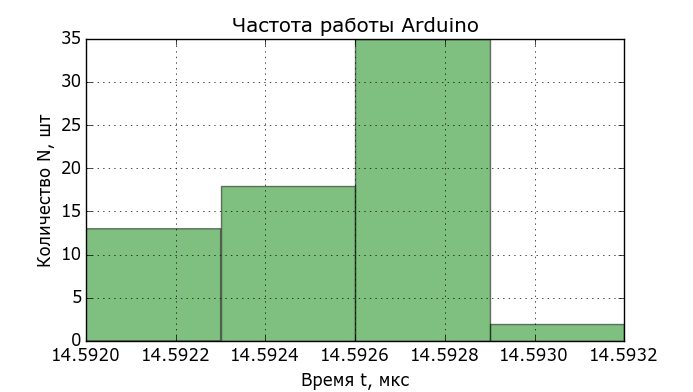
\includegraphics[width=.8\linewidth]{Figures/ardhist.png}
    \caption{Гистограмма измерений частоты Arduino}
    \label{fig:ardhist}
\end{figure}

Другими словами, дли включения и выключения одного выхода микроконтроллера \textbf{10000} раз нам понадобилось \textbf{145928} микросекунд, или \textbf{146} миллисекунд.

Одно включение и выключение выхода занимает $\frac{145928}{10000} = 14.5928$ микросекунд. Таким образом, \textbf{arduino} может выдавать сигнал с максимальной частотой

\begin{equation}
    \label{eq:freq1}
    \nu = \frac{n}{t} = \frac{10000}{145928 \cdot 10^{-6}} = 68526~\textrm{Гц} = 68.5~\textrm{кГц}
\end{equation}


    \subsection{Максимальная частота выхода atmega}
    Для того, чтобы повысить частоту сигнала, воспользуемся управлением непосредственно портами \textbf{ATmega}. Изменим в нашей программе строки

\begin{minted}[gobble=4,fontsize=\footnotesize]{c}
    digitalWrite(13, HIGH); //Turn on LED 13
    digitalWrite(13, LOW);  //Turn off LED 13
\end{minted}

на

\begin{minted}[gobble=4,fontsize=\footnotesize]{c}
    PORTB |= _BV(PORTB5);  //Turn on PORTB5
    PORTB &= ~_BV(PORTB5); //Turn off PORTB5
\end{minted}

PORTB5 является Pin 13 для Arduino UNO (ATmega328) и Pin 11 для Arduino MEGA 2560 (ATmega 2560). Диаграмма портов ATmega для Arduino представлена на рисунке~\ref{fig:a328diagram}.

\begin{figure}[ht]
    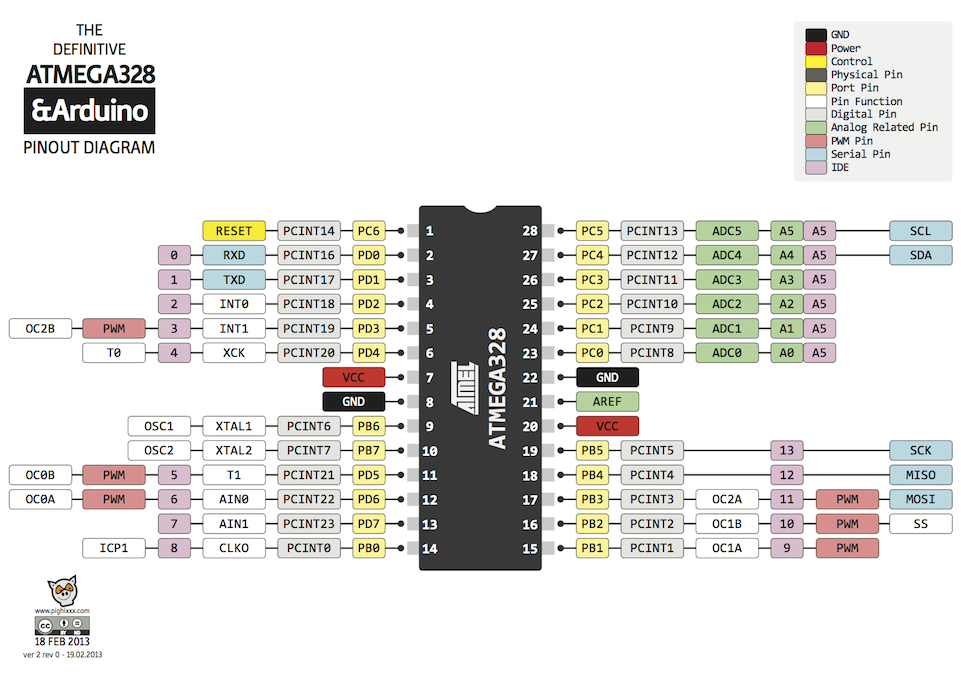
\includegraphics[width=1\linewidth]{Figures/a328diagram.png}
    \caption{Диаграмма портов ATmega328 для Arduino}
    \label{fig:a328diagram}
\end{figure}

В результате получаем значительный прирост скорости:

\begin{longtable}[c]{|c|c|}
    \caption{Результат работы напрямую с портами}
    \label{PortsResult}\\
    \hline
    \textbf{Количество, шт} & \textbf{Результат, мкс}\\
    \hline
    \endfirsthead
    \hline
    \textbf{Количество, шт} & \textbf{Результат, мкс}\\
    \hline
    \endhead
        1 & 6916\\
        \hline
        235 & 6940\\
        \hline
        328 & 6944\\
        \hline
        821 & 6948\\
        \hline
\end{longtable}

\begin{figure}[ht]
    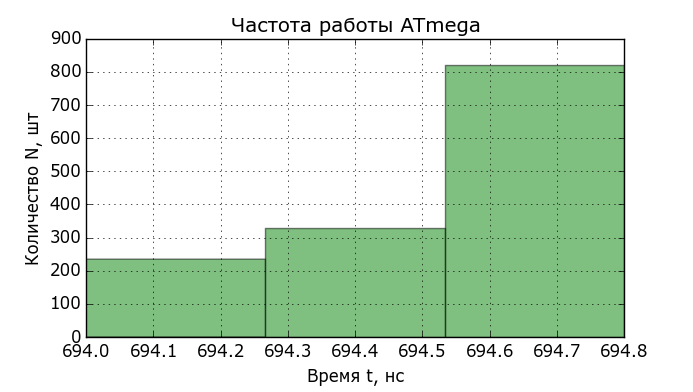
\includegraphics[width=.8\linewidth]{Figures/athist.png}
    \caption{Гистограмма измерений частоты ATmega}
    \label{fig:athist}
\end{figure}

То есть за счёт использования более низкого уровня взаимодействия с железом, мы добились увеличения скорости в $\frac{145928}{6948} = 21$ раз!

В итоге, максимальная скорость сигнала равна

\begin{equation}
    \label{eq:freq2}
    f = \frac{n}{t} = \frac{10000}{6948 \cdot 10^{-6}} = 1439263~\textrm{Гц} = 1.44~\textrm{МГц}
\end{equation}


    \subsection{Максимальная скорость бибиотеки virtualwire}
    \label{sec:virtualwirefreq}
    Библиотека VirtualWire представляет собой высокоуровневую надстройку над Arduino для удобной передачи сообщений на расстоянии путём радиосигнала. Так как сама библиотека сложна и содержит множество задержек, замерим непосредственно минимальное время отправки сигнала --- максимальную частоту работы VirtualWire.

В целях эксперимента напишем программу, которая будет посылать один ASCII-символ данных типа \textbf{char}, занимающий ровно 1 байт (8 бит). Для обеспечения максимальной скорости, не будем ждать пока сообщение будет полностью отправлено, а будем сразу посылать следующее (если это позволит нам сделать сама \textit{VirtualWire}):

\begin{minted}[gobble=4,fontsize=\footnotesize]{c}
    #include <VirtualWire.h>
    unsigned long initial = 0; //0 - 4,294,967,295
    unsigned long final = 0;
    int i; //-32,768 - 32,767

    int TX_PIN = 1;

    const char *msg = "1";
    uint8_t buf[VW_MAX_MESSAGE_LEN];
    uint8_t buflen = VW_MAX_MESSAGE_LEN;

    void setup(){
        Serial.begin(9600);

        vw_set_tx_pin(TX_PIN);
        vw_set_ppt_inverted(true);
        vw_setup(2000);
    }

    void loop(){
        initial = micros();
        for (i = 0; i < 10; i++){
            vw_send((uint8_t *)msg, strlen(msg));
            //vw_wait_tx(); //Wait for message gone
        }
        final = micros();
        Serial.println(final - initial);
        while (final > 1E7); //Stop after 10 seconds
    }
\end{minted}

На выходе получается:

\begin{longtable}[c]{|c|c|}
    \caption{Результат использования VirtualWire}
    \label{VirtualWireResult}\\
    \hline
    \textbf{Количество, шт} & \textbf{Результат, мкс}\\
    \hline
    \endfirsthead
    \hline
    \textbf{Количество, шт} & \textbf{Результат, мкс}\\
    \hline
    \endhead
        7 & 480536\\
        \hline
        6 & 480540\\
        \hline
        7 & 480544\\
        \hline
\end{longtable}

Можно заметить, что в этом испытании было проведено лишь 10 итераций, что в итоге даёт нам частоту, не превышающую:

\begin{equation}
    \label{eq:freq3}
    f = \frac{n}{t} = \frac{10}{480540 \cdot 10^{-6}} = 20~\textrm{Гц}
\end{equation}

По-сути, VirtualWire способна передавать данные с максимальными скоростями вплоть до скоростей датчиков (9600 Кбит/с для FS1000A), однако это скорость передачи цельного блока данных. При передачи одного байта задержки складываются из-за больших битовых затрат на инициализацию драйвера передачи данных, формирование <<шапки>> пакета и проверки надежности доставки данных.

Таким образом, для наших целей библиотека VirtualWire не подходит.


    \subsection{Максимальная скорость радиомодуля fs1000a}
    \label{sec:fs1000a}
    Радиопередающий модуль FS1000A представляет собой низкобюджетное устройство передачи радиосообщений (рисунок~\ref{fig:fs1000a}). Спецификация FS1000A представлена ниже~\cite{fs1000a:specs}:

\begin{figure}[ht]
    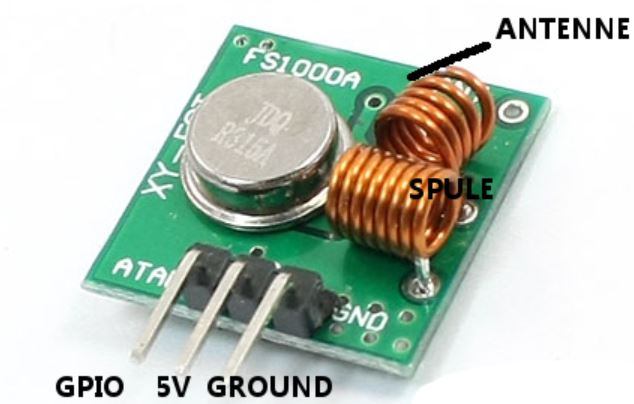
\includegraphics[width=.3\linewidth]{Figures/fs1000a.jpg}
    \caption{Радиопередатчик FS1000A}
    \label{fig:fs1000a}
\end{figure}

\begin{longtable}[c]{|c|c|}
    \caption{Спецификация модуля FS1000A}
    \label{tab:specs}\\
    \hline
    \textbf{Параметр} & \textbf{Значение}\\
    \hline
    \endfirsthead
    \hline
    \textbf{Параметр} & \textbf{Значение}\\
    \hline
    \endhead
        Входное напряжение & 2.5 -- 12 В\\
        \hline
        Тип модуляции & Амплитудная\\
        \hline
        Максимальная скорость передачи данных & 9.6 Кбит/с\\
        \hline
\end{longtable}

Скорость передачи данных в данном случае говорит, что за одну секунду можно передать блок данных размером в $\frac{9.6}{8} = 1.2$ Кб, или 9600 бит. Другими словами, если отправлять пачку длиной в 1 бит как полноценное сообщение с передатчика на приёмник, максимально доступной частотой для нас будет 9.6 КГц. Однако для надёжной передачи сообщения необходимо \textbf{как минимум} 3 бита: синхронизирующий бит, бит данных и ещё один бит данных, представляющий собой инверсию данных для подтверждения подлинности. Естественно, чем больше битов в синхронизирующем сообщении и в самом сообщении, тем надёжнее будет посылка.

Если взглянуть в справочник по передачи данных на физическом уровне (через UART), можно также заметить, что стандартное время передачи одного символа (12 бит) на скорости 9600 бит/с не превышает 1.25 мсек (рисунок~\ref{fig:mits})~\cite{mits:fx}:

\begin{figure}[ht]
    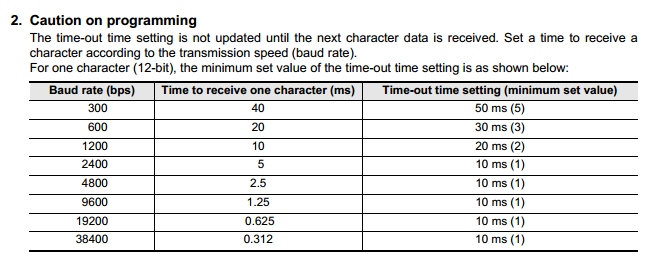
\includegraphics[width=1\linewidth]{Figures/mits.png}
    \caption{Скорость передачи данных (PLC Data Communication Manual)}
    \label{fig:mits}
\end{figure}


    % Экспериментальные данные по RaspberryPI со ссылкой наверх.

    \newpage
    \subsection{Итоги}
    Учитывая идеальную частоту библиотеки VirualWire в 20 Гц (глава~\ref{sec:virtualwirefreq}), получим сокращение времени ожидания с 4 часов до 12 минут. Однако 20 Гц --- это лишь идеальная частота передачи сообщения. Т. к. сообщение летит в обе стороны, частота уменьшается в 2 раза (10 Гц). Учитывая некоторые задержки и помехи во время передачи, получим частоту менее 10 Гц.

Как было показано в главе~\ref{sec:fs1000a}, частота используемого в данном проекте передатчика достигает 9.6 кГц, что в идеале позволит нам сократить время накопления с 4 часов до двух секунд.

Учитывая, что время накопления в 1 минуту уже будет достаточным условием рациональности проекта, рассчитаем необходимую частоту работы устройства:

$$f = \frac{t_1}{1~\textrm{мин}} = \frac{252~\textrm{мин}}{1~\textrm{мин}} = 252~\textrm{Гц},$$

где $t_1$ --- время накопления с частотой в 1 Гц.

Соответственно, на данном этапе стоит задача создания собственной библиотеки передачи данных, приспособленной для использования на больших частотах, или же поиск более быстрой библиотеки, аналогичной VirtualWire (например, RadioHead).


\section{АНАЛИЗ РЕЗУЛЬТАТОВ}
В результате моделирования были получены нерелевантные данные, т. к. частота работы имеющегося оборудования гораздо ниже необходимых (глава~\ref{sec:taskfreq}).

Как было показано в главе~\ref{sec:mitigation}, для целей измерения Time of Flight выгоднее использовать более высокочастотные, микропроцессорные технологии, работающие на гигагерцовых частотах. Также, Wi-Fi-диапазон частот (2.4ГГц) для этой цели подойдёт больше, чем свободная полоса 433 МГц.

Для повышения надёжности всей системы, необходимо увеличить размер передаваемого сообщения, что сказывается на требованиях к скоростям радиодатчиков.

Получившиеся в главе~\ref{sec:taskfreq} задержки можно вычислить аналитически, используя данные платформы Arduino/ATMega (процессора ATMega 328) о количестве тактов, необходимых для проведения определённых операций. Библиотека WirtualWire (приложение В) содержит множество команд, CRC-проверку и формирование достаточно большго пакета бит для стабильной отправки сообщения, поэтому в ней возникают наибольшие задержки.

Общие задержки складываются из трёх факторов:

\begin{enumerate}
    \item Инициализация радиопередатчика и приём сообщения радиоприёмником.
    \item Передача электрических импульсов на входы и выходы микроконтроллера, задержки в портах, наводки.
    \item Задержки, связанные с выполнением инструкций микропроцессором.
\end{enumerate}

Первая группа задержек определяется характеристиками приёмника и передатчика. Так как в проекте был использован дешёвый передатчик FS1000A со скоростью передачи данных не более 9600 Кбит/с, задержки на инициализацию радиопередатчика и приём сообщения могут быть достаточно большими чтоб учитывать их в расчёте общей задержки. Также, на скорость и качество радиопередачи будет влиять длина и правильность антенны.

На вторую группу задержек влияют такие факторы, как наличие белого шума, расстояние между контактами и т. д. Вторая группа, как правило, наименьшая из трёх. При поверхностной оценке задержек эту группу можно опустить, однако для построения точного Time of Flight устройства с наилучшими параметрами работы необходимо учесть все данные при проектировании печатной платы.

Третья группа задержек является основной, минимизировать которую представляется возможным путём оптимизации программного модуля. При использовании ARM-ядра, количество инструкций можно сократить. Когда умножение двух чисел в AVR-ядре займёт 5 инструкций, в ARM-ядре оно будет вычислено в одну инструкцию. Проведя анализ программного кода, можно рассчитать общую задержку, связанную с выполнением инструкций в AVR-ядре. После этого, можно получить задержку, связанную с радиопередачей сообщения, используя экспериментальные данные об общей задержке всей передачи.

% Анализ теоретических и практических результатов.
% Конечные расчёты.

\section{ЭКОНОМИКА}
\newpage
.
\newpage

    \subsection{Расчёт капитальных вложений потребителей сравниваемых моделей оборудования}
    \newpage

    \subsection{Расчёт годовых эксплуатационных издержек потребителей при использовании сравниваемых моделей оборудования}
    \newpage
    .
    \newpage

    \subsection{Расчёт полезного эффекта при переходе на новую модель оборудования}
    \newpage

    \subsection{Расчёт основных технико-экономических показателей для сравниваемых моделей оборудования и определение верхнего предела цены разрабатываемой модели оборудования}
    \newpage
    .
    \newpage

    \subsection{Расчёт и построение графиков зависимостей}
    \newpage
    .
    \newpage
    .
    \newpage
    .
    \newpage

\section{ОХРАНА ТРУДА}

    \subsection{Производственная санитария, техника безопасности и пожарная профилактика}
    \newpage

        \subsubsection{Метеоусловия}
        \newpage
        .
        \newpage

        \subsubsection{Вентиляция и отопление}
        \newpage

        \subsubsection{Освещение}
        \newpage

        \subsubsection{Шум}
        \newpage

        \subsubsection{Электробезопасность}

        \subsubsection{Излучение}
        \newpage
        .
        \newpage

        \subsubsection{Пожарная безопасность}
        \newpage

    \subsection{Безопасность эксплуатации радиоэлектронного оборудования}
    \newpage
    .
    \newpage
    .
    \newpage

\section{ЭКОЛОГИЯ}
\subsection{Воздействие радиоактивного излучения на электронные системы}

Проникающая радиация и радиоактивное заражение (ионизирующие излучения) могут изменять качество и свойства некоторых материалов, используемых в электронных системах, что приводит к сбоям и даже отказам в работе этих систем.

Особенно подвержены воздействию ионизирующих излучений полупроводниковые, газоразрядные, вакуумные приборы, некоторые типы конденсаторов и резисторов, органические материалы. Из неорганических материалов наиболее подвержены воздействию ионизирующих излучений оптические стекла, которые под действием излучений могут существенно увеличивать оптическую плотность~\cite{econ1}.

Современные интегральные микросхемы находят все более широкое применение в радиоэлектронной аппаратуре различного рода технических объектов, работающих в условиях воздействия проникающей радиации. Эти условия могут возникать при попадании объекта в зону действия источников ионизирующего излучения техногенного происхождения или при расположении вблизи ядерных силовых и энергетических установок, а на аппаратуру космических объектов воздействуют ионизирующие излучения космического пространства и радиационных поясов Земли. При этом радиоэлектронная аппаратура (РЭА) может подвергаться воздействию следующих уровней радиации:

\begin{itemize}
    \item от ядерного взрыва --- потоку нейтронов до 1015 на $\textrm{см}^2$ и гамма-квантов с экспозиционной дозой до 106 Рад при мощности дозы до 1013 Р/с;
    \item вблизи ядерных реакторов --- потоку нейтронов 1012--1015 и дозе гамма-квантов до 107 Рад~\cite{econ1}.
\end{itemize}

Высокая стоимость радиоэлектронных систем обуславливает особо жесткие требования к безотказности элементной базы радиоэлектронной аппаратуры и, в первую очередь, к микросхемам различного функционального назначения. Действительно, отказ одной микросхемы в условиях воздействия вышеперечисленных дестабилизирующих факторов может повлечь за собой выход из строя всего сложного и дорогостоящего объекта, причем последствия подобного отказа не всегда предсказуемы. Поэтому задача гарантированного обеспечения радиационной стойкости интегральных микросхем и аппаратуры на их основе является исключительно актуальной.

\subsection{Оценка устройчивости проектируемой системы к радиоактивному излучению}

Радиационная стойкость --- способность материалов сохранять исходный химический состав, структуру и свойства в процессе и (или) после воздействия ионизирующих излучений (ИИ).

Радиационная стойкость существенно зависит от вида радиации, величины и мощности поглощенной дозы, режима облучения (непрерывное или импульсное, кратковременное или длительное), условий эксплуатации материала (температура, высокое давление, механические нагрузки, магнитное или электрическое поле), размеров образца материала и других факторов. На практике изменение свойств материала сопоставляется с величиной, характеризующей величину воздействующего излучения, например с потоком (флюенсом) нейтронов или поглощенной дозой ИИ. Количественной характеристикой часто служит также максимальное (предельное) значение поглощенной дозы и (или) мощности поглощенной дозы излучения, при котором материал становится непригодным для конкретных условий применения или до заданной степени меняет значение характерного параметра. Обычно проводят ускоренные радиационные испытания в лабораторных условиях, имитирующих эксплуатационные.

Возникающие в результате радиационно-индукционных процессов ионы и свободные электроны могут участвовать в сложных цепях физико-химических превращений (образование новых молекул и свободных радикалов, изменение кристаллической структуры и др.), совокупно приводящих к изменению механических, электрических, материальных, оптических и других свойств материалов. Изменения в материалах могут быть обратимыми или необратимыми и произойти как непосредственно вслед за радиационным воздействием, так и в течение длительного времени после акта облучения.

Радиационная стойкость неорганических веществ зависит от кристаллической структуры и типа химической связи. Наиболее стойки ионные кристаллы. Плотные структуры с высокой симметрией наиболее устойчивы к воздействию излучений. Для стекол характерно изменение прозрачности и появление окраски; возможна кристаллизация. Силикаты начинают изменять свойства после облучения флюенсом нейтронов ~1019 $\textrm{см}^2$. В результате облучения происходят: анизотропное расширение кристалла, аморфизация его структуры, уменьшение плотности, упругости, теплопроводности и других свойств. Оксиды при облучении нейтронами меняют свои свойства аналогично силикатам, но в меньшей степени. В свойствах бетонов существующие изменения отсутствуют при облучении флюенсом нейтронов до $3 \cdot 1019 \textrm{см}^2$.

Свойства металлов изменяются в зависимости от повреждений кристаллической решетки. Одиночные дефекты обычно упрочняют металл, но снижают его пластичность. Электрическое сопротивление металлов или сплавов возрастает за счет образования дефектов, хотя в сплавах возможно и уменьшение электрического сопротивления, если радиационное воздействие приводит к упорядочению структуры. В полупроводниках всегда имеется некоторая равновесная при определенной температуре концентрация точечных дефектов. Под действием облучения она увеличивается, что приводит к изменению электрических и оптических свойств полупроводников~\cite{econ2}.

Радиационная стойкость органических материалов принято определять величиной радиационно-химического выхода продуктов радиолиза, образующихся при поглощении 100 эВ энергии ИИ. Взаимодействие ИИ с орг. соед. сопровождается образованием промежуточных активных частиц, деструкцией, окислением, сшиванием, газообразованием, деполимеризацией (для полимеров) и т. д. Низкой радиационной стойкостью обладают вещества, содержащие связи С—F, С — Si, С—О. Наличие в молекуле двойных и сопряженных связей, ароматических колец и гетероциклов увеличивает радиационную стойкость. Наиболее значительные изменения структуры полимерных материалов под действием ИИ происходят при деструкции или сшивании молекул полимера.

Радиационная стойкость, в т. ч. полимеров, зависит и от количества растворенного в них О2 воздуха и скорости его поступления из окружающей среды; в его присутствии происходит радиационно-химическое окисление вещества. В результате этого существенно изменяются химическая и термическая стойкость веществ, предел прочности и модуль упругости, диэлектрическая проницаемость, электрическая прочность и электрическая проводимость.

Обратимые изменения в органических материалах обусловлены установлением стационарного равновесия между генерированием нестабильных продуктов радиолиза и их гибелью и зависят от мощности дозы. Так, электрическое сопротивление органических изоляционных материалов с увеличением мощности дозы падает на несколько порядков. При больших дозах снижение остаточного электрического сопротивления носит необратимый характер. У многих полимерных материалов, облученных дозами до 106 Гр, исходная электрическая проводимость меняется в несколько раз. При дозе 104 Гр необратимые изменения, как правило, незначительны. В органических полимерных материалах может возникать послерадиационное старение, которое обусловлено в основном химическими реакциями образовавшихся свободных радикалов с О2 воздуха. Радиационная стойкость полимерных диэлектриков ограничивается, как правило, их механическими свойствами, т. к. они становятся хрупкими и теряют способность нести механические нагрузки после доз, не вызывающих существенных изменений электрических св-в.

В таблице~\ref{tab:ecology} представлены значения дозы облучения, вызывающие заметные (до 50\%) изменения свойств некоторых материалов.

\begin{longtable}[c]{|c|c|}
    \caption{Радиационная стойкость некоторых материалов}
    \label{tab:ecology}\\
    \hline
    \textbf{Материал} & \textbf{Радиационная стойкость}\\
    \hline
    \endfirsthead
    \hline
    \textbf{Материал} & \textbf{Доза, Гр}\\
    \hline
    \endhead
        Стекло & $5 \cdot 10^7$ ($5 \cdot 10^{17}$)\\
        \hline
        Керамика & $5 \cdot 10^7$ -- $3 \cdot 10^{20}$ ($10^{20}$ -- $3 \cdot 10^{20}$)\\
        \hline
        Сталь конструкционная & $5 \cdot 10^7$ -- ($> 10^{19}$)\\
        \hline
        Бетон & ($10^{20}$ -- $5 \cdot 10^{20}$)\\
        \hline
        Кремний (транзисторы) & $10^3$ -- $10^5$ ($3 \cdot 10^{11}$ -- $10^{13}$)\\
        \hline
        Германий (транзисторы) & $10^4$ -- $10^6$ ($4 \cdot 10^{12}$ -- $10^{14}$)\\
        \hline
        Графит & $5 \cdot 10^8$ -- $3 \cdot 10^9$\\
        \hline
        Ферриты & $2 \cdot 10^4$ -- $3 \cdot 10^9$\\
        \hline
        Фотоплёнка & 0,01 -- 0,2\\
        \hline
\end{longtable}

Значения без скобок относятся к дозе $\gamma$-излучения, в скобках --- к флюенсу быстрых нейтронов, $\textrm{см}^{-2}$.

Для повышения радиационной стойкости обычно используют пассивную защиту (экранирование), физико-химические модификацию материала, радиационно-термическую обработку. Использование защитного экранирования снижает степень воздействия ИИ на материал. Таким путем в весьма широких пределах можно "повысить" стойкость любого материала. При физико-химической модификации в материал вводят добавки --- например, антиоксиданты, таким путем радиационная стойкость может быть повышена в 7-20 раз. Предварительная радиационно-термическая обработка-облучение и отжиг позволяет увеличить радиационную стойкость металлических материалов в 10-50 раз.


\section*{\centerline{ЗАКЛЮЧЕНИЕ}}
\addcontentsline{toc}{section}{ЗАКЛЮЧЕНИЕ}
В ходе выполнения дипломного проекта был исследован процесс передачи информации по радиоканалу и определение расстояния методом Time of Flight. Были проанализированы погрешности и задержки, возникающие как в аппаратной, так и в программной части. Были выявлены основные недостатки и предложены пути увеличения точности и скорости работы. Был сконструирован абстрактный модуль определения расстояния методом Time of Flight (аппаратная и программная часть), а также предложено оптимальное оборудование для достижения наилучших результатов.

Исследуемая система обеспечивает определение расстояния между узлами технологического процесса для дальнейшего использования этих данных в диспетчерских (SCADA) системах.

% Выводы и предложения (кратко, списком).

\newpage
\addcontentsline{toc}{section}{СПИСОК ИСПОЛЬЗОВАННОЙ ЛИТЕРАТУРЫ}
\bibliography{web,books}

\section*{\centerline{ПРИЛОЖЕНИЕ А}} %Arduino reference design.
\addcontentsline{toc}{section}{ПРИЛОЖЕНИЕ А}
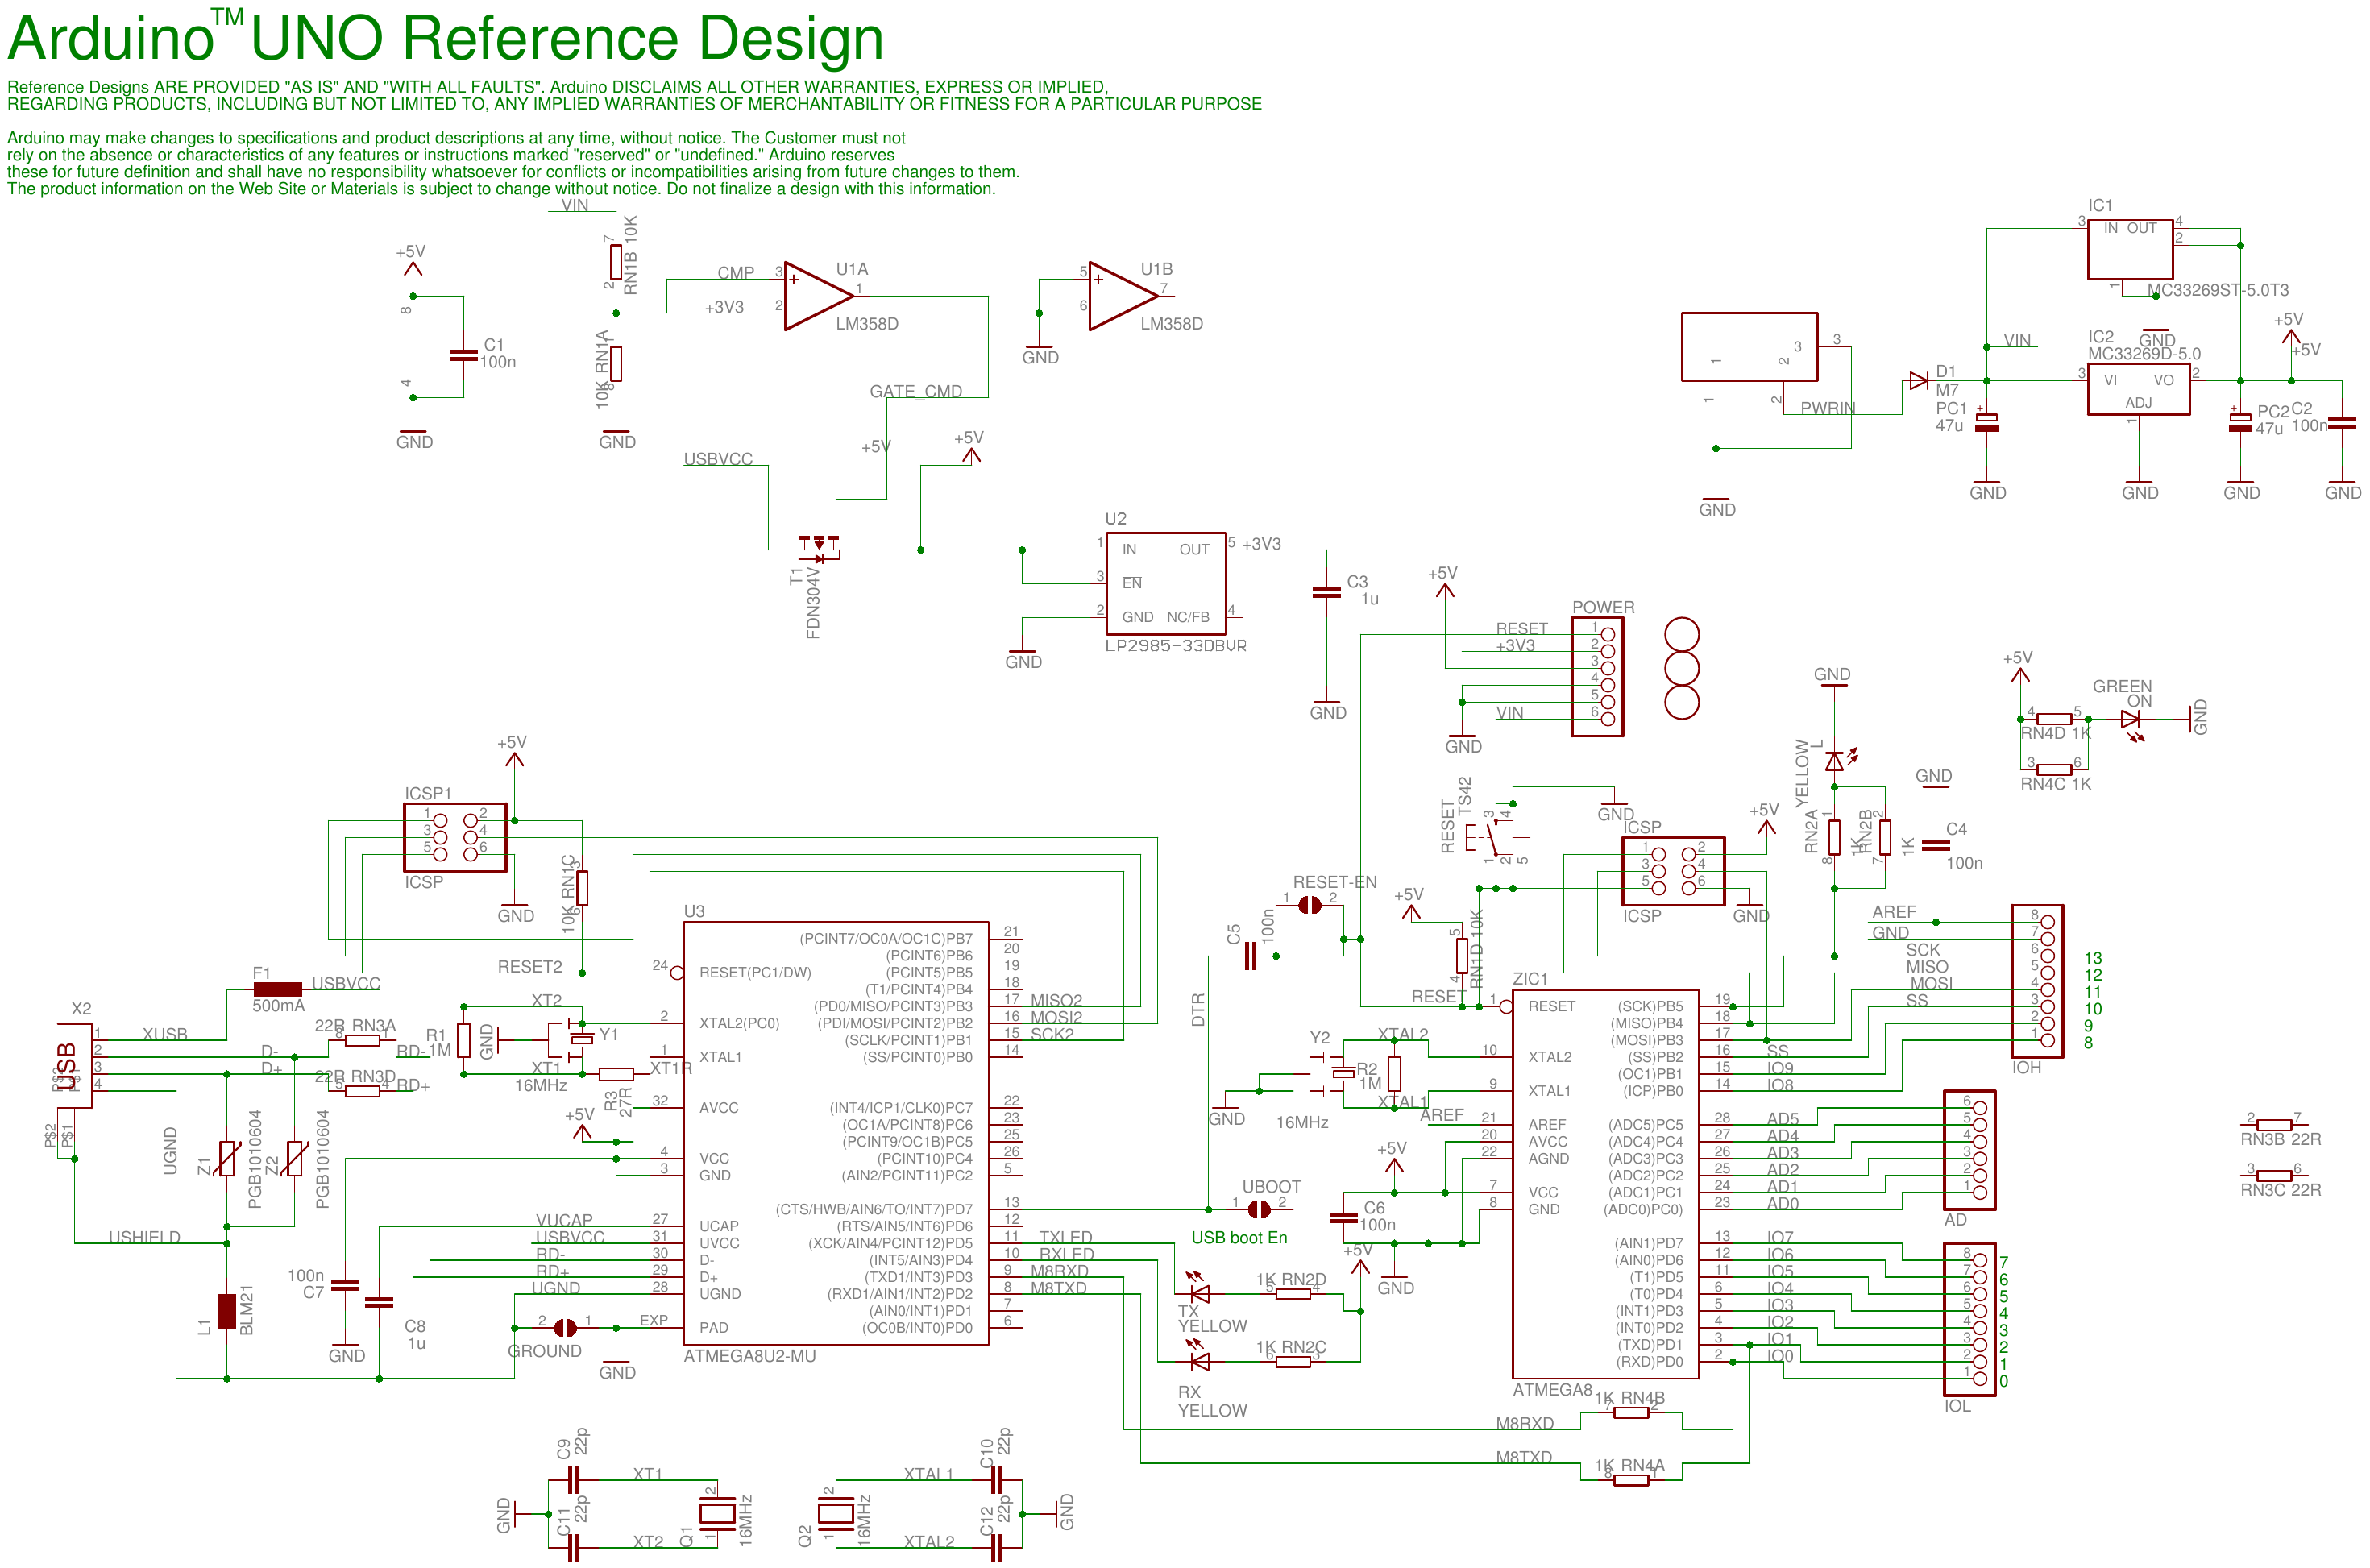
\includegraphics[angle=90,width=.9\linewidth]{Figures/arduinodatasheet.png}


\section*{\centerline{ПРИЛОЖЕНИЕ Б}} %Схемотехника подключения.
\addcontentsline{toc}{section}{ПРИЛОЖЕНИЕ Б}
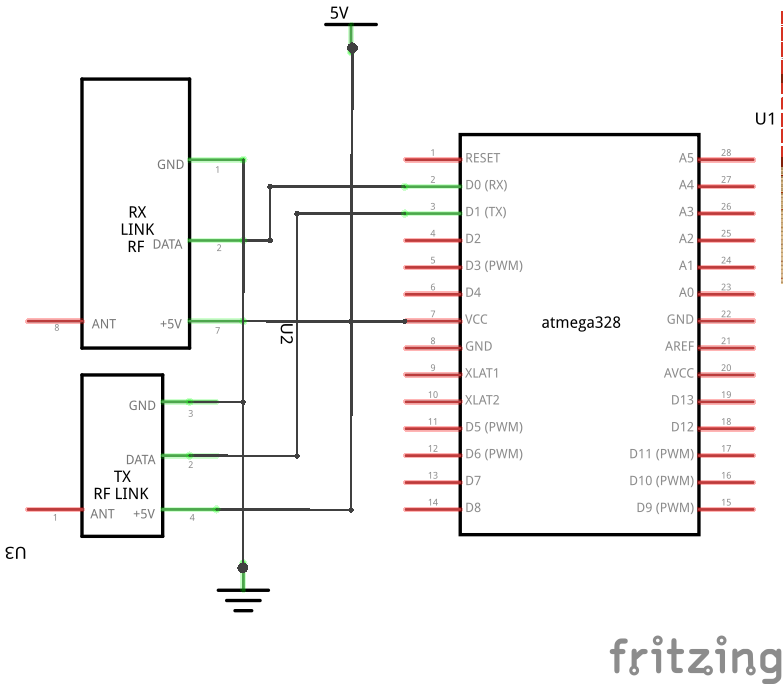
\includegraphics[width=.9\linewidth]{Figures/circscheme.png}


\section*{\centerline{ПРИЛОЖЕНИЕ В}} %Библиотека VirtualWire.
\addcontentsline{toc}{section}{ПРИЛОЖЕНИЕ В}
\begin{minted}[gobble=4,fontsize=\footnotesize,breaklines=true]{cpp}
    // VirtualWire.h
    //
    // Virtual Wire implementation for Arduino
    // See the README file in this directory fdor documentation
    // 
    // Author: Mike McCauley (mikem@airspayce.com) DO NOT CONTACT THE AUTHOR DIRECTLY: USE THE LISTS
    // Copyright (C) 2008 Mike McCauley
    // $Id: VirtualWire.h,v 1.6 2013/02/14 22:02:11 mikem Exp mikem $

    #ifndef VirtualWire_h
    #define VirtualWire_h

    #include <stdlib.h>
    #if defined(ARDUINO)
     #if ARDUINO >= 100
      #include <Arduino.h>
     #else
      #include <wiring.h>
     #endif
    #elif defined(__MSP430G2452__) || defined(__MSP430G2553__) // LaunchPad specific
     #include "legacymsp430.h"
     #include "Energia.h"
    #else // error
     #error Platform not defined
    #endif

    // These defs cause trouble on some versions of Arduino
    #undef abs
    #undef double
    #undef round

    /// Maximum number of bytes in a message, counting the byte count and FCS
    #define VW_MAX_MESSAGE_LEN 30

    /// The maximum payload length
    #define VW_MAX_PAYLOAD VW_MAX_MESSAGE_LEN-3

    /// The size of the receiver ramp. Ramp wraps modulu this number
    #define VW_RX_RAMP_LEN 160

    /// Number of samples per bit
    #define VW_RX_SAMPLES_PER_BIT 8

    // Ramp adjustment parameters
    // Standard is if a transition occurs before VW_RAMP_TRANSITION (80) in the ramp,
    // the ramp is retarded by adding VW_RAMP_INC_RETARD (11)
    // else by adding VW_RAMP_INC_ADVANCE (29)
    // If there is no transition it is adjusted by VW_RAMP_INC (20)
    /// Internal ramp adjustment parameter
    #define VW_RAMP_INC (VW_RX_RAMP_LEN/VW_RX_SAMPLES_PER_BIT)
    /// Internal ramp adjustment parameter
    #define VW_RAMP_TRANSITION VW_RX_RAMP_LEN/2
    /// Internal ramp adjustment parameter
    #define VW_RAMP_ADJUST 9
    /// Internal ramp adjustment parameter
    #define VW_RAMP_INC_RETARD (VW_RAMP_INC-VW_RAMP_ADJUST)
    /// Internal ramp adjustment parameter
    #define VW_RAMP_INC_ADVANCE (VW_RAMP_INC+VW_RAMP_ADJUST)

    /// Outgoing message bits grouped as 6-bit words
    /// 36 alternating 1/0 bits, followed by 12 bits of start symbol
    /// Followed immediately by the 4-6 bit encoded byte count, 
    /// message buffer and 2 byte FCS
    /// Each byte from the byte count on is translated into 2x6-bit words
    /// Caution, each symbol is transmitted LSBit first, 
    /// but each byte is transmitted high nybble first
    #define VW_HEADER_LEN 8

    // Cant really do this as a real C++ class, since we need to have 
    // an ISR
    extern "C"
    {
        /// Set the digital IO pin to be for transmit data. 
        /// This pin will only be accessed if
        /// the transmitter is enabled
        /// \param[in] pin The Arduino pin number for transmitting data. Defaults to 12.
        extern void vw_set_tx_pin(uint8_t pin);

        /// Set the digital IO pin to be for receive data.
        /// This pin will only be accessed if
        /// the receiver is enabled
        /// \param[in] pin The Arduino pin number for receiving data. Defaults to 11.
        extern void vw_set_rx_pin(uint8_t pin);

        // Set the digital IO pin to enable the transmitter (press to talk, PTT)'
        /// This pin will only be accessed if
        /// the transmitter is enabled
        /// \param[in] pin The Arduino pin number to enable the transmitter. Defaults to 10.
        extern void vw_set_ptt_pin(uint8_t pin);

        /// By default the PTT pin goes high when the transmitter is enabled.
        /// This flag forces it low when the transmitter is enabled.
        /// \param[in] inverted True to invert PTT
        extern void vw_set_ptt_inverted(uint8_t inverted);

        /// Initialise the VirtualWire software, to operate at speed bits per second
        /// Call this one in your setup() after any vw_set_* calls
        /// Must call vw_rx_start() before you will get any messages
        /// \param[in] speed Desired speed in bits per second
        extern void vw_setup(uint16_t speed);

        /// Start the Phase Locked Loop listening to the receiver
        /// Must do this before you can receive any messages
        /// When a message is available (good checksum or not), vw_have_message();
        /// will return true.
        extern void vw_rx_start();

        /// Stop the Phase Locked Loop listening to the receiver
        /// No messages will be received until vw_rx_start() is called again
        /// Saves interrupt processing cycles
        extern void vw_rx_stop();

        /// Returns the state of the
        /// transmitter
        /// \return true if the transmitter is active else false
        extern uint8_t vx_tx_active();

        /// Block until the transmitter is idle
        /// then returns
        extern void vw_wait_tx();

        /// Block until a message is available
        /// then returns
        extern void vw_wait_rx();

        /// Block until a message is available or for a max time
        /// \param[in] milliseconds Maximum time to wait in milliseconds.
        /// \return true if a message is available, false if the wait timed out.
        extern uint8_t vw_wait_rx_max(unsigned long milliseconds);

        /// Send a message with the given length. Returns almost immediately,
        /// and message will be sent at the right timing by interrupts
        /// \param[in] buf Pointer to the data to transmit
        /// \param[in] len Number of octetes to transmit
        /// \return true if the message was accepted for transmission, false if the message is too long (>VW_MAX_MESSAGE_LEN - 3)
        extern uint8_t vw_send(uint8_t* buf, uint8_t len);

        // Returns true if an unread message is available
        /// \return true if a message is available to read
        extern uint8_t vw_have_message();

        // If a message is available (good checksum or not), copies
        // up to *len octets to buf.
        /// \param[in] buf Pointer to location to save the read data (must be at least *len bytes.
        /// \param[in,out] len Available space in buf. Will be set to the actual number of octets read
        /// \return true if there was a message and the checksum was good
        extern uint8_t vw_get_message(uint8_t* buf, uint8_t* len);
    }

    /// @example client.pde
    /// Client side of simple client/server pair using VirtualWire

    /// @example server.pde
    /// Server side of simple client/server pair using VirtualWire

    /// @example transmitter.pde
    /// Transmitter side of simple one-way transmitter->receiver pair using VirtualWire

    /// @example receiver.pde
    /// Transmitter side of simple one-way transmitter->receiver pair using VirtualWire

    #endif
\end{minted}

\begin{minted}[gobble=4,fontsize=\footnotesize,breaklines=true]{cpp}
    // VirtualWire.cpp
    //
    // Virtual Wire implementation for Arduino
    // See the README file in this directory fdor documentation
    // See also
    // ASH Transceiver Software Designer's Guide of 2002.08.07
    //   http://www.rfm.com/products/apnotes/tr_swg05.pdf
    //
    // Changes:
    // 1.5 2008-05-25: fixed a bug that could prevent messages with certain
    //  bytes sequences being received (false message start detected)
    // 1.6 2011-09-10: Patch from David Bath to prevent unconditional reenabling of the receiver
    //  at end of transmission.
    //
    // Author: Mike McCauley (mikem@airspayce.com)
    // Copyright (C) 2008 Mike McCauley
    // $Id: VirtualWire.cpp,v 1.9 2013/02/14 22:02:11 mikem Exp mikem $


    #if defined(ARDUINO)
     #if (ARDUINO < 100)
      #include "WProgram.h"
     #endif
    #elif defined(__MSP430G2452__) || defined(__MSP430G2553__) // LaunchPad specific
     #include "legacymsp430.h"
     #include "Energia.h"
    #else // error
     #error Platform not defined
    #endif

    #include "VirtualWire.h"
    #include <util/crc16.h>


    static uint8_t vw_tx_buf[(VW_MAX_MESSAGE_LEN * 2) + VW_HEADER_LEN] 
         = {0x2a, 0x2a, 0x2a, 0x2a, 0x2a, 0x2a, 0x38, 0x2c};

    // Number of symbols in vw_tx_buf to be sent;
    static uint8_t vw_tx_len = 0;

    // Index of the next symbol to send. Ranges from 0 to vw_tx_len
    static uint8_t vw_tx_index = 0;

    // Bit number of next bit to send
    static uint8_t vw_tx_bit = 0;

    // Sample number for the transmitter. Runs 0 to 7 during one bit interval
    static uint8_t vw_tx_sample = 0;

    // Flag to indicated the transmitter is active
    static volatile uint8_t vw_tx_enabled = 0;

    // Total number of messages sent
    static uint16_t vw_tx_msg_count = 0;

    // The digital IO pin number of the press to talk, enables the transmitter hardware
    static uint8_t vw_ptt_pin = 10;
    static uint8_t vw_ptt_inverted = 0;

    // The digital IO pin number of the receiver data
    static uint8_t vw_rx_pin = 11;

    // The digital IO pin number of the transmitter data
    static uint8_t vw_tx_pin = 12;

    // Current receiver sample
    static uint8_t vw_rx_sample = 0;

    // Last receiver sample
    static uint8_t vw_rx_last_sample = 0;

    // PLL ramp, varies between 0 and VW_RX_RAMP_LEN-1 (159) over 
    // VW_RX_SAMPLES_PER_BIT (8) samples per nominal bit time. 
    // When the PLL is synchronised, bit transitions happen at about the
    // 0 mark. 
    static uint8_t vw_rx_pll_ramp = 0;

    // This is the integrate and dump integral. If there are <5 0 samples in the PLL cycle
    // the bit is declared a 0, else a 1
    static uint8_t vw_rx_integrator = 0;

    // Flag indictate if we have seen the start symbol of a new message and are
    // in the processes of reading and decoding it
    static uint8_t vw_rx_active = 0;

    // Flag to indicate that a new message is available
    static volatile uint8_t vw_rx_done = 0;

    // Flag to indicate the receiver PLL is to run
    static uint8_t vw_rx_enabled = 0;

    // Last 12 bits received, so we can look for the start symbol
    static uint16_t vw_rx_bits = 0;

    // How many bits of message we have received. Ranges from 0 to 12
    static uint8_t vw_rx_bit_count = 0;

    // The incoming message buffer
    static uint8_t vw_rx_buf[VW_MAX_MESSAGE_LEN];

    // The incoming message expected length
    static uint8_t vw_rx_count = 0;

    // The incoming message buffer length received so far
    static volatile uint8_t vw_rx_len = 0;

    // Number of bad messages received and dropped due to bad lengths
    static uint8_t vw_rx_bad = 0;

    // Number of good messages received
    static uint8_t vw_rx_good = 0;

    // 4 bit to 6 bit symbol converter table
    // Used to convert the high and low nybbles of the transmitted data
    // into 6 bit symbols for transmission. Each 6-bit symbol has 3 1s and 3 0s 
    // with at most 3 consecutive identical bits
    static uint8_t symbols[] =
    {
        0xd,  0xe,  0x13, 0x15, 0x16, 0x19, 0x1a, 0x1c, 
        0x23, 0x25, 0x26, 0x29, 0x2a, 0x2c, 0x32, 0x34
    };

    // Cant really do this as a real C++ class, since we need to have 
    // an ISR
    extern "C"
    {

    // Compute CRC over count bytes.
    // This should only be ever called at user level, not interrupt level
    uint16_t vw_crc(uint8_t *ptr, uint8_t count)
    {
        uint16_t crc = 0xffff;

        while (count-- > 0) 
        crc = _crc_ccitt_update(crc, *ptr++);
        return crc;
    }

    // Convert a 6 bit encoded symbol into its 4 bit decoded equivalent
    uint8_t vw_symbol_6to4(uint8_t symbol)
    {
        uint8_t i;
        
        // Linear search :-( Could have a 64 byte reverse lookup table?
        for (i = 0; i < 16; i++)
        if (symbol == symbols[i]) return i;
        return 0; // Not found
    }

    // Set the output pin number for transmitter data
    void vw_set_tx_pin(uint8_t pin)
    {
        vw_tx_pin = pin;
    }

    // Set the pin number for input receiver data
    void vw_set_rx_pin(uint8_t pin)
    {
        vw_rx_pin = pin;
    }

    // Set the output pin number for transmitter PTT enable
    void vw_set_ptt_pin(uint8_t pin)
    {
        vw_ptt_pin = pin;
    }

    // Set the ptt pin inverted (low to transmit)
    void vw_set_ptt_inverted(uint8_t inverted)
    {
        vw_ptt_inverted = inverted;
    }

    // Called 8 times per bit period
    // Phase locked loop tries to synchronise with the transmitter so that bit 
    // transitions occur at about the time vw_rx_pll_ramp is 0;
    // Then the average is computed over each bit period to deduce the bit value
    void vw_pll()
    {
        // Integrate each sample
        if (vw_rx_sample)
        vw_rx_integrator++;

        if (vw_rx_sample != vw_rx_last_sample)
        {
        // Transition, advance if ramp > 80, retard if < 80
        vw_rx_pll_ramp += ((vw_rx_pll_ramp < VW_RAMP_TRANSITION) 
                   ? VW_RAMP_INC_RETARD 
                   : VW_RAMP_INC_ADVANCE);
        vw_rx_last_sample = vw_rx_sample;
        }
        else
        {
        // No transition
        // Advance ramp by standard 20 (== 160/8 samples)
        vw_rx_pll_ramp += VW_RAMP_INC;
        }
        if (vw_rx_pll_ramp >= VW_RX_RAMP_LEN)
        {
        // Add this to the 12th bit of vw_rx_bits, LSB first
        // The last 12 bits are kept
        vw_rx_bits >>= 1;

        // Check the integrator to see how many samples in this cycle were high.
        // If < 5 out of 8, then its declared a 0 bit, else a 1;
        if (vw_rx_integrator >= 5)
            vw_rx_bits |= 0x800;

        vw_rx_pll_ramp -= VW_RX_RAMP_LEN;
        vw_rx_integrator = 0; // Clear the integral for the next cycle

        if (vw_rx_active)
        {
            // We have the start symbol and now we are collecting message bits,
            // 6 per symbol, each which has to be decoded to 4 bits
            if (++vw_rx_bit_count >= 12)
            {
            // Have 12 bits of encoded message == 1 byte encoded
            // Decode as 2 lots of 6 bits into 2 lots of 4 bits
            // The 6 lsbits are the high nybble
            uint8_t this_byte = 
                (vw_symbol_6to4(vw_rx_bits & 0x3f)) << 4 
                | vw_symbol_6to4(vw_rx_bits >> 6);

            // The first decoded byte is the byte count of the following message
            // the count includes the byte count and the 2 trailing FCS bytes
            // REVISIT: may also include the ACK flag at 0x40
            if (vw_rx_len == 0)
            {
                // The first byte is the byte count
                // Check it for sensibility. It cant be less than 4, since it
                // includes the bytes count itself and the 2 byte FCS
                vw_rx_count = this_byte;
                if (vw_rx_count < 4 || vw_rx_count > VW_MAX_MESSAGE_LEN)
                {
                // Stupid message length, drop the whole thing
                vw_rx_active = false;
                vw_rx_bad++;
                            return;
                }
            }
            vw_rx_buf[vw_rx_len++] = this_byte;

            if (vw_rx_len >= vw_rx_count)
            {
                // Got all the bytes now
                vw_rx_active = false;
                vw_rx_good++;
                vw_rx_done = true; // Better come get it before the next one starts
            }
            vw_rx_bit_count = 0;
            }
        }
        // Not in a message, see if we have a start symbol
        else if (vw_rx_bits == 0xb38)
        {
            // Have start symbol, start collecting message
            vw_rx_active = true;
            vw_rx_bit_count = 0;
            vw_rx_len = 0;
            vw_rx_done = false; // Too bad if you missed the last message
        }
        }
    }

    // Common function for setting timer ticks @ prescaler values for speed
    // Returns prescaler index into {0, 1, 8, 64, 256, 1024} array
    // and sets nticks to compare-match value if lower than max_ticks
    // returns 0 & nticks = 0 on fault
    static uint8_t _timer_calc(uint16_t speed, uint16_t max_ticks, uint16_t *nticks)
    {
        // Clock divider (prescaler) values - 0/3333: error flag
        uint16_t prescalers[] = {0, 1, 8, 64, 256, 1024, 3333};
        uint8_t prescaler=0; // index into array & return bit value
        unsigned long ulticks; // calculate by ntick overflow

        // Div-by-zero protection
        if (speed == 0)
        {
            // signal fault
            *nticks = 0;
            return 0;
        }

        // test increasing prescaler (divisor), decreasing ulticks until no overflow
        for (prescaler=1; prescaler < 7; prescaler += 1)
        {
            // Amount of time per CPU clock tick (in seconds)
            float clock_time = (1.0 / (float(F_CPU) / float(prescalers[prescaler])));
            // Fraction of second needed to xmit one bit
            float bit_time = ((1.0 / float(speed)) / 8.0);
            // number of prescaled ticks needed to handle bit time @ speed
            ulticks = long(bit_time / clock_time);
            // Test if ulticks fits in nticks bitwidth (with 1-tick safety margin)
            if ((ulticks > 1) && (ulticks < max_ticks))
            {
                break; // found prescaler
            }
            // Won't fit, check with next prescaler value
        }

        // Check for error
        if ((prescaler == 6) || (ulticks < 2) || (ulticks > max_ticks))
        {
            // signal fault
            *nticks = 0;
            return 0;
        }

        *nticks = ulticks;
        return prescaler;
    }

    #if defined(__arm__) && defined(CORE_TEENSY)
      // This allows the AVR interrupt code below to be run from an
      // IntervalTimer object.  It must be above vw_setup(), so the
      // the TIMER1_COMPA_vect function name is defined.
      #ifdef SIGNAL
      #undef SIGNAL
      #endif
      #define SIGNAL(f) void f(void)
      #ifdef TIMER1_COMPA_vect
      #undef TIMER1_COMPA_vect
      #endif
      void TIMER1_COMPA_vect(void);
    #endif


    // Speed is in bits per sec RF rate
    #if defined(__MSP430G2452__) || defined(__MSP430G2553__) // LaunchPad specific
    void vw_setup(uint16_t speed)
    {
        // Calculate the counter overflow count based on the required bit speed
        // and CPU clock rate
        uint16_t ocr1a = (F_CPU / 8UL) / speed;
            
        // This code is for Energia/MSP430
        TA0CCR0 = ocr1a;				// Ticks for 62,5 us
        TA0CTL = TASSEL_2 + MC_1;       // SMCLK, up mode
        TA0CCTL0 |= CCIE;               // CCR0 interrupt enabled
            
        // Set up digital IO pins
        pinMode(vw_tx_pin, OUTPUT);
        pinMode(vw_rx_pin, INPUT);
        pinMode(vw_ptt_pin, OUTPUT);
        digitalWrite(vw_ptt_pin, vw_ptt_inverted);
    }	

    #elif defined (ARDUINO) // Arduino specific
    void vw_setup(uint16_t speed)
    {
        uint16_t nticks; // number of prescaled ticks needed
        uint8_t prescaler; // Bit values for CS0[2:0]

    #ifdef __AVR_ATtiny85__
        // figure out prescaler value and counter match value
        prescaler = _timer_calc(speed, (uint8_t)-1, &nticks);
        if (!prescaler)
        {
            return; // fault
        }

        TCCR0A = 0;
        TCCR0A = _BV(WGM01); // Turn on CTC mode / Output Compare pins disconnected

        // convert prescaler index to TCCRnB prescaler bits CS00, CS01, CS02
        TCCR0B = 0;
        TCCR0B = prescaler; // set CS00, CS01, CS02 (other bits not needed)

        // Number of ticks to count before firing interrupt
        OCR0A = uint8_t(nticks);

        // Set mask to fire interrupt when OCF0A bit is set in TIFR0
        TIMSK |= _BV(OCIE0A);

    #elif defined(__arm__) && defined(CORE_TEENSY)
        // on Teensy 3.0 (32 bit ARM), use an interval timer
        IntervalTimer *t = new IntervalTimer();
        t->begin(TIMER1_COMPA_vect, 125000.0 / (float)(speed));

    #else // ARDUINO
        // This is the path for most Arduinos
        // figure out prescaler value and counter match value
        prescaler = _timer_calc(speed, (uint16_t)-1, &nticks);
        if (!prescaler)
        {
            return; // fault
        }

        TCCR1A = 0; // Output Compare pins disconnected
        TCCR1B = _BV(WGM12); // Turn on CTC mode

        // convert prescaler index to TCCRnB prescaler bits CS10, CS11, CS12
        TCCR1B |= prescaler;

        // Caution: special procedures for setting 16 bit regs
        // is handled by the compiler
        OCR1A = nticks;
        // Enable interrupt
    #ifdef TIMSK1
        // atmega168
        TIMSK1 |= _BV(OCIE1A);
    #else
        // others
        TIMSK |= _BV(OCIE1A);
    #endif // TIMSK1

    #endif // __AVR_ATtiny85__

        // Set up digital IO pins
        pinMode(vw_tx_pin, OUTPUT);
        pinMode(vw_rx_pin, INPUT);
        pinMode(vw_ptt_pin, OUTPUT);
        digitalWrite(vw_ptt_pin, vw_ptt_inverted);
    }

    #endif // ARDUINO

    // Start the transmitter, call when the tx buffer is ready to go and vw_tx_len is
    // set to the total number of symbols to send
    void vw_tx_start()
    {
        vw_tx_index = 0;
        vw_tx_bit = 0;
        vw_tx_sample = 0;

        // Enable the transmitter hardware
        digitalWrite(vw_ptt_pin, true ^ vw_ptt_inverted);

        // Next tick interrupt will send the first bit
        vw_tx_enabled = true;
    }

    // Stop the transmitter, call when all bits are sent
    void vw_tx_stop()
    {
        // Disable the transmitter hardware
        digitalWrite(vw_ptt_pin, false ^ vw_ptt_inverted);
        digitalWrite(vw_tx_pin, false);

        // No more ticks for the transmitter
        vw_tx_enabled = false;
    }

    // Enable the receiver. When a message becomes available, vw_rx_done flag
    // is set, and vw_wait_rx() will return.
    void vw_rx_start()
    {
        if (!vw_rx_enabled)
        {
        vw_rx_enabled = true;
        vw_rx_active = false; // Never restart a partial message
        }
    }

    // Disable the receiver
    void vw_rx_stop()
    {
        vw_rx_enabled = false;
    }

    // Return true if the transmitter is active
    uint8_t vx_tx_active()
    {
        return vw_tx_enabled;
    }

    // Wait for the transmitter to become available
    // Busy-wait loop until the ISR says the message has been sent
    void vw_wait_tx()
    {
        while (vw_tx_enabled)
        ;
    }

    // Wait for the receiver to get a message
    // Busy-wait loop until the ISR says a message is available
    // can then call vw_get_message()
    void vw_wait_rx()
    {
        while (!vw_rx_done)
        ;
    }

    // Wait at most max milliseconds for the receiver to receive a message
    // Return the truth of whether there is a message
    uint8_t vw_wait_rx_max(unsigned long milliseconds)
    {
        unsigned long start = millis();

        while (!vw_rx_done && ((millis() - start) < milliseconds))
        ;
        return vw_rx_done;
    }

    // Wait until transmitter is available and encode and queue the message
    // into vw_tx_buf
    // The message is raw bytes, with no packet structure imposed
    // It is transmitted preceded a byte count and followed by 2 FCS bytes
    uint8_t vw_send(uint8_t* buf, uint8_t len)
    {
        uint8_t i;
        uint8_t index = 0;
        uint16_t crc = 0xffff;
        uint8_t *p = vw_tx_buf + VW_HEADER_LEN; // start of the message area
        uint8_t count = len + 3; // Added byte count and FCS to get total number of bytes

        if (len > VW_MAX_PAYLOAD)
        return false;

        // Wait for transmitter to become available
        vw_wait_tx();

        // Encode the message length
        crc = _crc_ccitt_update(crc, count);
        p[index++] = symbols[count >> 4];
        p[index++] = symbols[count & 0xf];

        // Encode the message into 6 bit symbols. Each byte is converted into 
        // 2 6-bit symbols, high nybble first, low nybble second
        for (i = 0; i < len; i++)
        {
        crc = _crc_ccitt_update(crc, buf[i]);
        p[index++] = symbols[buf[i] >> 4];
        p[index++] = symbols[buf[i] & 0xf];
        }

        // Append the fcs, 16 bits before encoding (4 6-bit symbols after encoding)
        // Caution: VW expects the _ones_complement_ of the CCITT CRC-16 as the FCS
        // VW sends FCS as low byte then hi byte
        crc = ~crc;
        p[index++] = symbols[(crc >> 4)  & 0xf];
        p[index++] = symbols[crc & 0xf];
        p[index++] = symbols[(crc >> 12) & 0xf];
        p[index++] = symbols[(crc >> 8)  & 0xf];

        // Total number of 6-bit symbols to send
        vw_tx_len = index + VW_HEADER_LEN;

        // Start the low level interrupt handler sending symbols
        vw_tx_start();

        return true;
    }

    // Return true if there is a message available
    uint8_t vw_have_message()
    {
        return vw_rx_done;
    }

    // Get the last message received (without byte count or FCS)
    // Copy at most *len bytes, set *len to the actual number copied
    // Return true if there is a message and the FCS is OK
    uint8_t vw_get_message(uint8_t* buf, uint8_t* len)
    {
        uint8_t rxlen;
        
        // Message available?
        if (!vw_rx_done)
        return false;
        
        // Wait until vw_rx_done is set before reading vw_rx_len
        // then remove bytecount and FCS
        rxlen = vw_rx_len - 3;
        
        // Copy message (good or bad)
        if (*len > rxlen)
        *len = rxlen;
        memcpy(buf, vw_rx_buf + 1, *len);
        
        vw_rx_done = false; // OK, got that message thanks
        
        // Check the FCS, return goodness
        return (vw_crc(vw_rx_buf, vw_rx_len) == 0xf0b8); // FCS OK?
    }

    // This is the interrupt service routine called when timer1 overflows
    // Its job is to output the next bit from the transmitter (every 8 calls)
    // and to call the PLL code if the receiver is enabled
    //ISR(SIG_OUTPUT_COMPARE1A)
    #if defined (ARDUINO) // Arduino specific

    #ifdef __AVR_ATtiny85__
    SIGNAL(TIM0_COMPA_vect)
    #else // Assume Arduino Uno (328p or similar)

    SIGNAL(TIMER1_COMPA_vect)
    #endif // __AVR_ATtiny85__

    {
        if (vw_rx_enabled && !vw_tx_enabled)
        vw_rx_sample = digitalRead(vw_rx_pin);
        
        // Do transmitter stuff first to reduce transmitter bit jitter due 
        // to variable receiver processing
        if (vw_tx_enabled && vw_tx_sample++ == 0)
        {
        // Send next bit
        // Symbols are sent LSB first
        // Finished sending the whole message? (after waiting one bit period 
        // since the last bit)
        if (vw_tx_index >= vw_tx_len)
        {
            vw_tx_stop();
            vw_tx_msg_count++;
        }
        else
        {
            digitalWrite(vw_tx_pin, vw_tx_buf[vw_tx_index] & (1 << vw_tx_bit++));
            if (vw_tx_bit >= 6)
            {
            vw_tx_bit = 0;
            vw_tx_index++;
            }
        }
        }
        if (vw_tx_sample > 7)
        vw_tx_sample = 0;
        
        if (vw_rx_enabled && !vw_tx_enabled)
        vw_pll();
    }
    #elif defined(__MSP430G2452__) || defined(__MSP430G2553__) // LaunchPad specific
    void vw_Int_Handler()
    {
        if (vw_rx_enabled && !vw_tx_enabled)
        vw_rx_sample = digitalRead(vw_rx_pin);
        
        // Do transmitter stuff first to reduce transmitter bit jitter due 
        // to variable receiver processing
        if (vw_tx_enabled && vw_tx_sample++ == 0)
        {
        // Send next bit
        // Symbols are sent LSB first
        // Finished sending the whole message? (after waiting one bit period 
        // since the last bit)
        if (vw_tx_index >= vw_tx_len)
        {
            vw_tx_stop();
            vw_tx_msg_count++;
        }
        else
        {
            digitalWrite(vw_tx_pin, vw_tx_buf[vw_tx_index] & (1 << vw_tx_bit++));
            if (vw_tx_bit >= 6)
            {
            vw_tx_bit = 0;
            vw_tx_index++;
            }
        }
        }
        if (vw_tx_sample > 7)
        vw_tx_sample = 0;
        
        if (vw_rx_enabled && !vw_tx_enabled)
        vw_pll();
    }

    interrupt(TIMER0_A0_VECTOR) Timer_A_int(void) 
    {
        vw_Int_Handler();
    };

    #endif


    }
\end{minted}

\begin{minted}[gobble=4,fontsize=\footnotesize, breaklines=true]{cpp}
    // util/crc16.h
    #ifndef _UTIL_CRC16_H_
    #define _UTIL_CRC16_H_

    #include <stdint.h>

    #define lo8(x) ((x)&0xff) 
    #define hi8(x) ((x)>>8)

        uint16_t crc16_update(uint16_t crc, uint8_t a)
        {
        int i;

        crc ^= a;
        for (i = 0; i < 8; ++i)
        {
            if (crc & 1)
            crc = (crc >> 1) ^ 0xA001;
            else
            crc = (crc >> 1);
        }

        return crc;
        }

        uint16_t crc_xmodem_update (uint16_t crc, uint8_t data)
        {
            int i;

            crc = crc ^ ((uint16_t)data << 8);
            for (i=0; i<8; i++)
            {
                if (crc & 0x8000)
                    crc = (crc << 1) ^ 0x1021;
                else
                    crc <<= 1;
            }

            return crc;
        }
        uint16_t _crc_ccitt_update (uint16_t crc, uint8_t data)
        {
            data ^= lo8 (crc);
            data ^= data << 4;

            return ((((uint16_t)data << 8) | hi8 (crc)) ^ (uint8_t)(data >> 4) 
                    ^ ((uint16_t)data << 3));
        }

        uint8_t _crc_ibutton_update(uint8_t crc, uint8_t data)
        {
        uint8_t i;

        crc = crc ^ data;
        for (i = 0; i < 8; i++)
        {
            if (crc & 0x01)
                crc = (crc >> 1) ^ 0x8C;
            else
                crc >>= 1;
        }

        return crc;
        }


    #endif /* _UTIL_CRC16_H_ */
\end{minted}

